%\mychapter{6}{Results}

\section{Results}
In this section, we report our results on noisy synthetic data using diffusion maps with the $l_{1}$ distance. We compare our results with those obtained via PCA, a popular linear dimensionality technique. Figure \ref{fig:DiffMaps_PCA_on_Prevtime_FR} (right column) shows that diffusion maps  with $l_{1}$ distance appears to capture the animal's circular motion better than PCA when applied on firing rate data. Using previous time data, diffusion maps with $l_{1}$ distance appears to outperform PCA (see the left column of Figure  \ref{fig:DiffMaps_PCA_on_Prevtime_FR}).
We also see that using previous time data captures changes in spike timing
as the animal makes 4 laps around the circle.\\

\begin{figure}[H]
        \centering
        \begin{subfigure}[b]{0.475\textwidth}
            \centering
            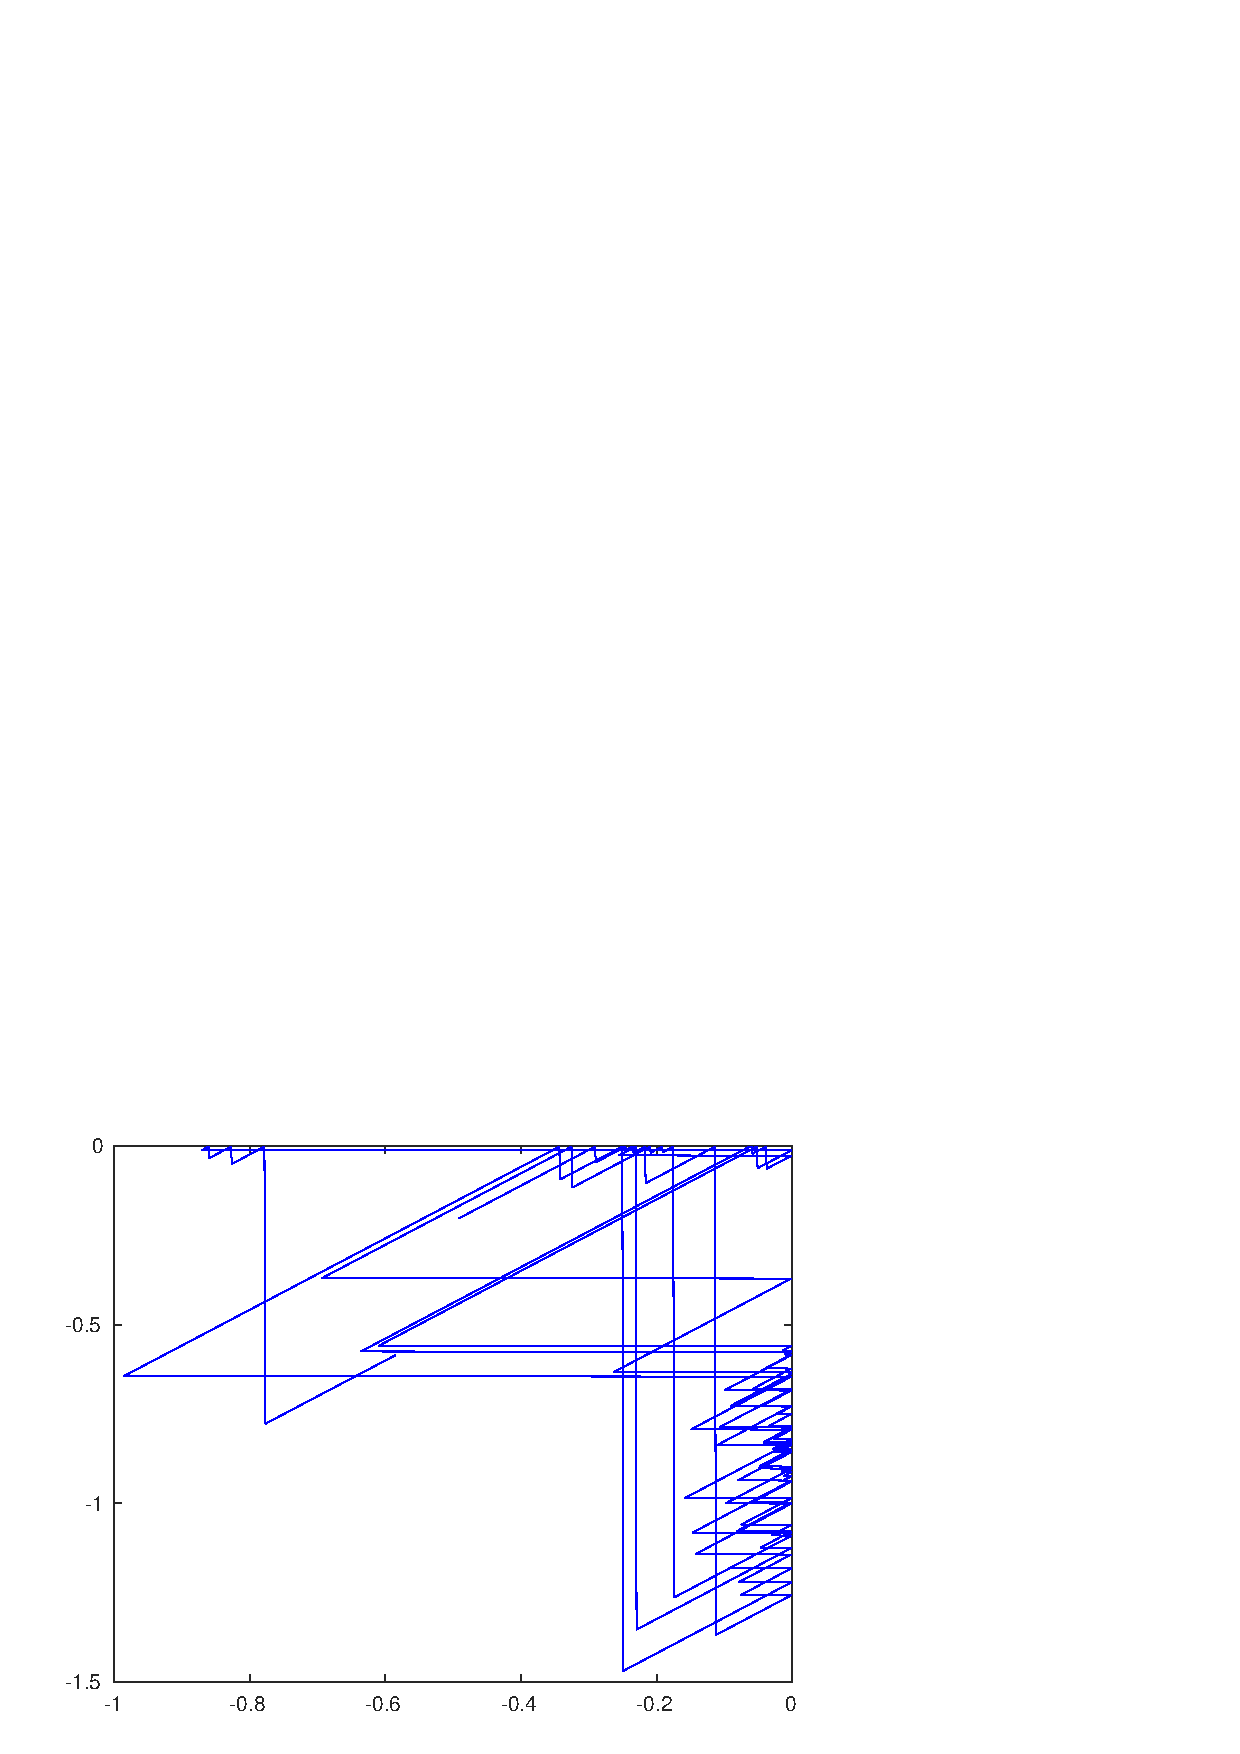
\includegraphics[width=\textwidth]{/home/tesylvia/Oral_Sept_2017/images/FinalOralPlots/SyntheticOralPaper/SimPrevtime.pdf}
            \caption[Simulated prevtime]%
            {{\small Simulated previous time data (Prevtime)}}    
            \label{fig:Prevtime in 3D}
        \end{subfigure}
        \hfill
        \begin{subfigure}[b]{0.475\textwidth}  
            \centering 
            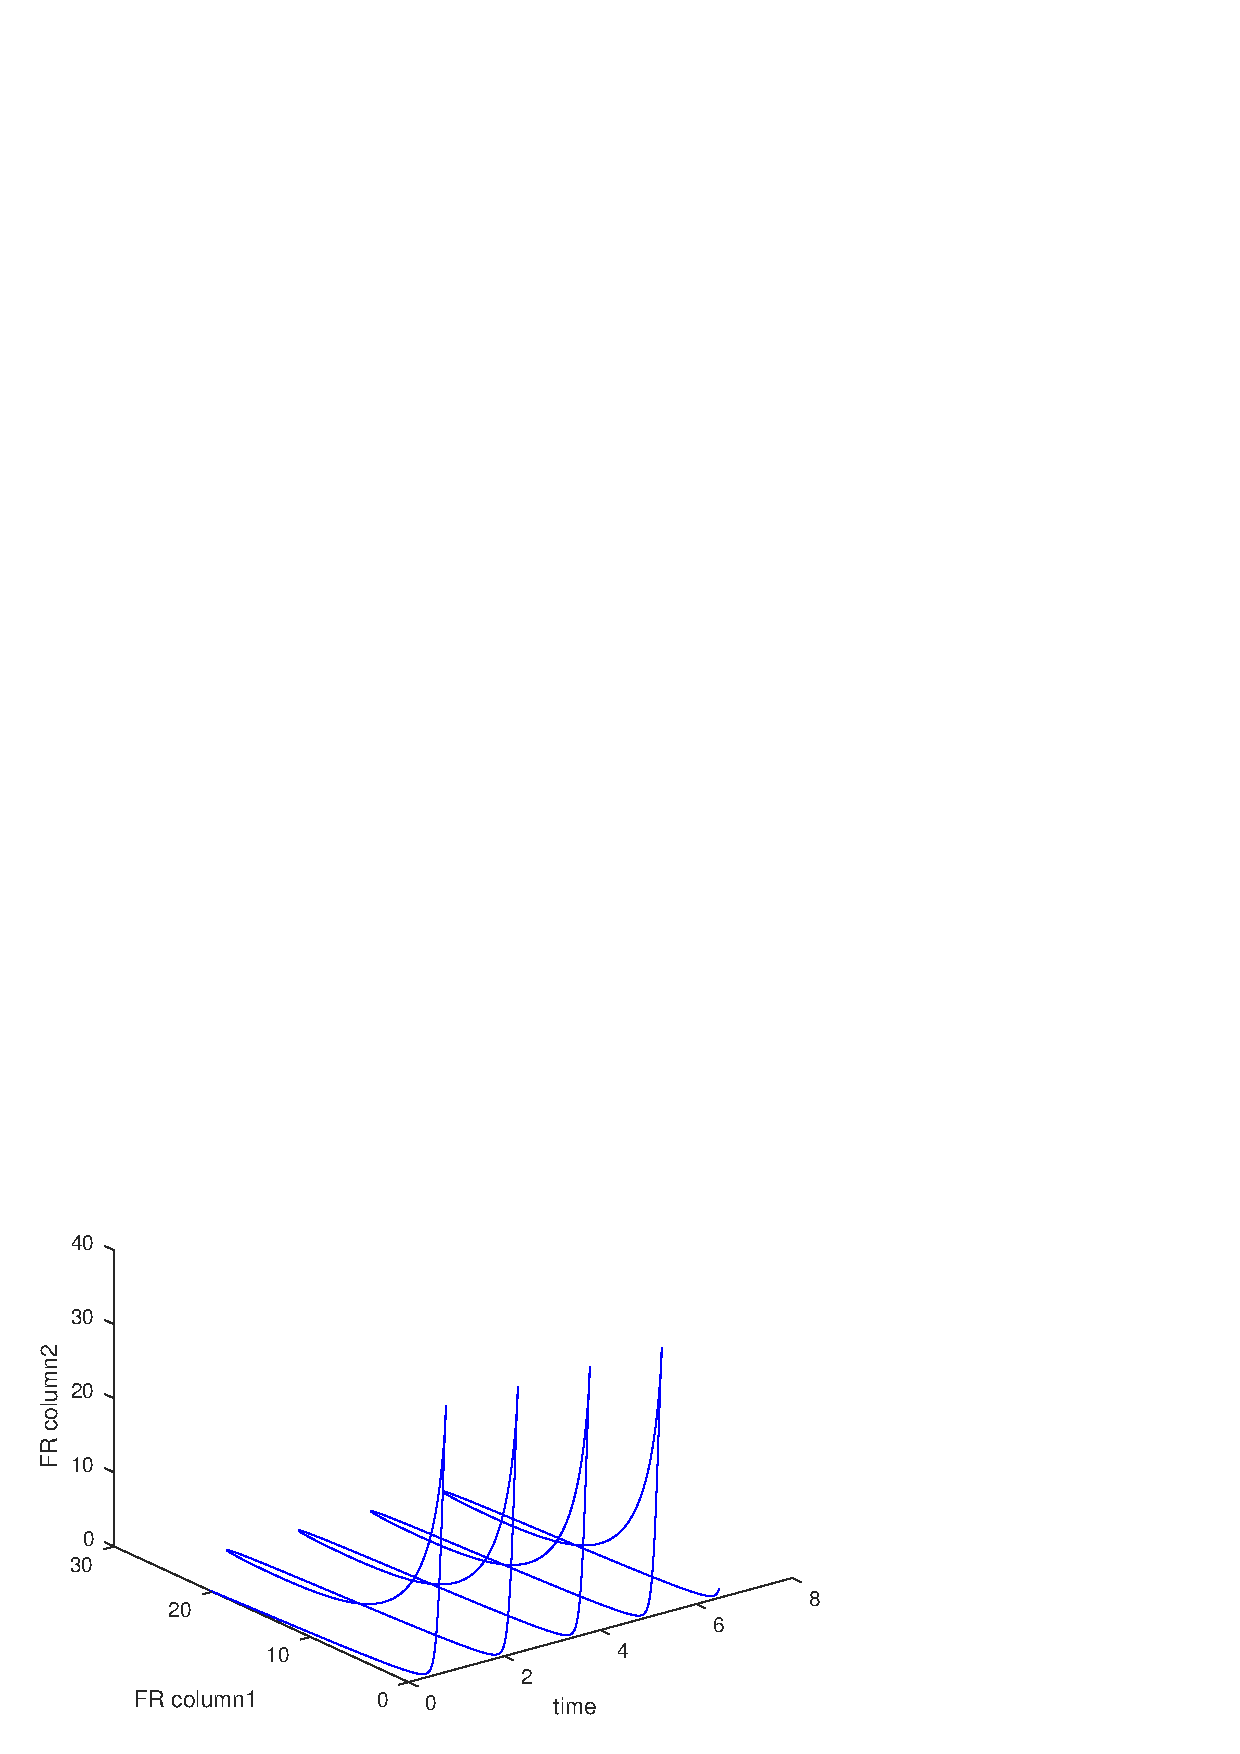
\includegraphics[width=\textwidth]{/home/tesylvia/Oral_Sept_2017/images/FinalOralPlots/SyntheticOralPaper/SimFiringRate-with-Time.pdf}
            \caption[]%
            {{\small Simulated firing rate data (FR)}}    
            \label{fig:Sim animal position in 3D}
        \end{subfigure}
        \vskip\baselineskip
        \begin{subfigure}[b]{0.475\textwidth}   
            \centering 
            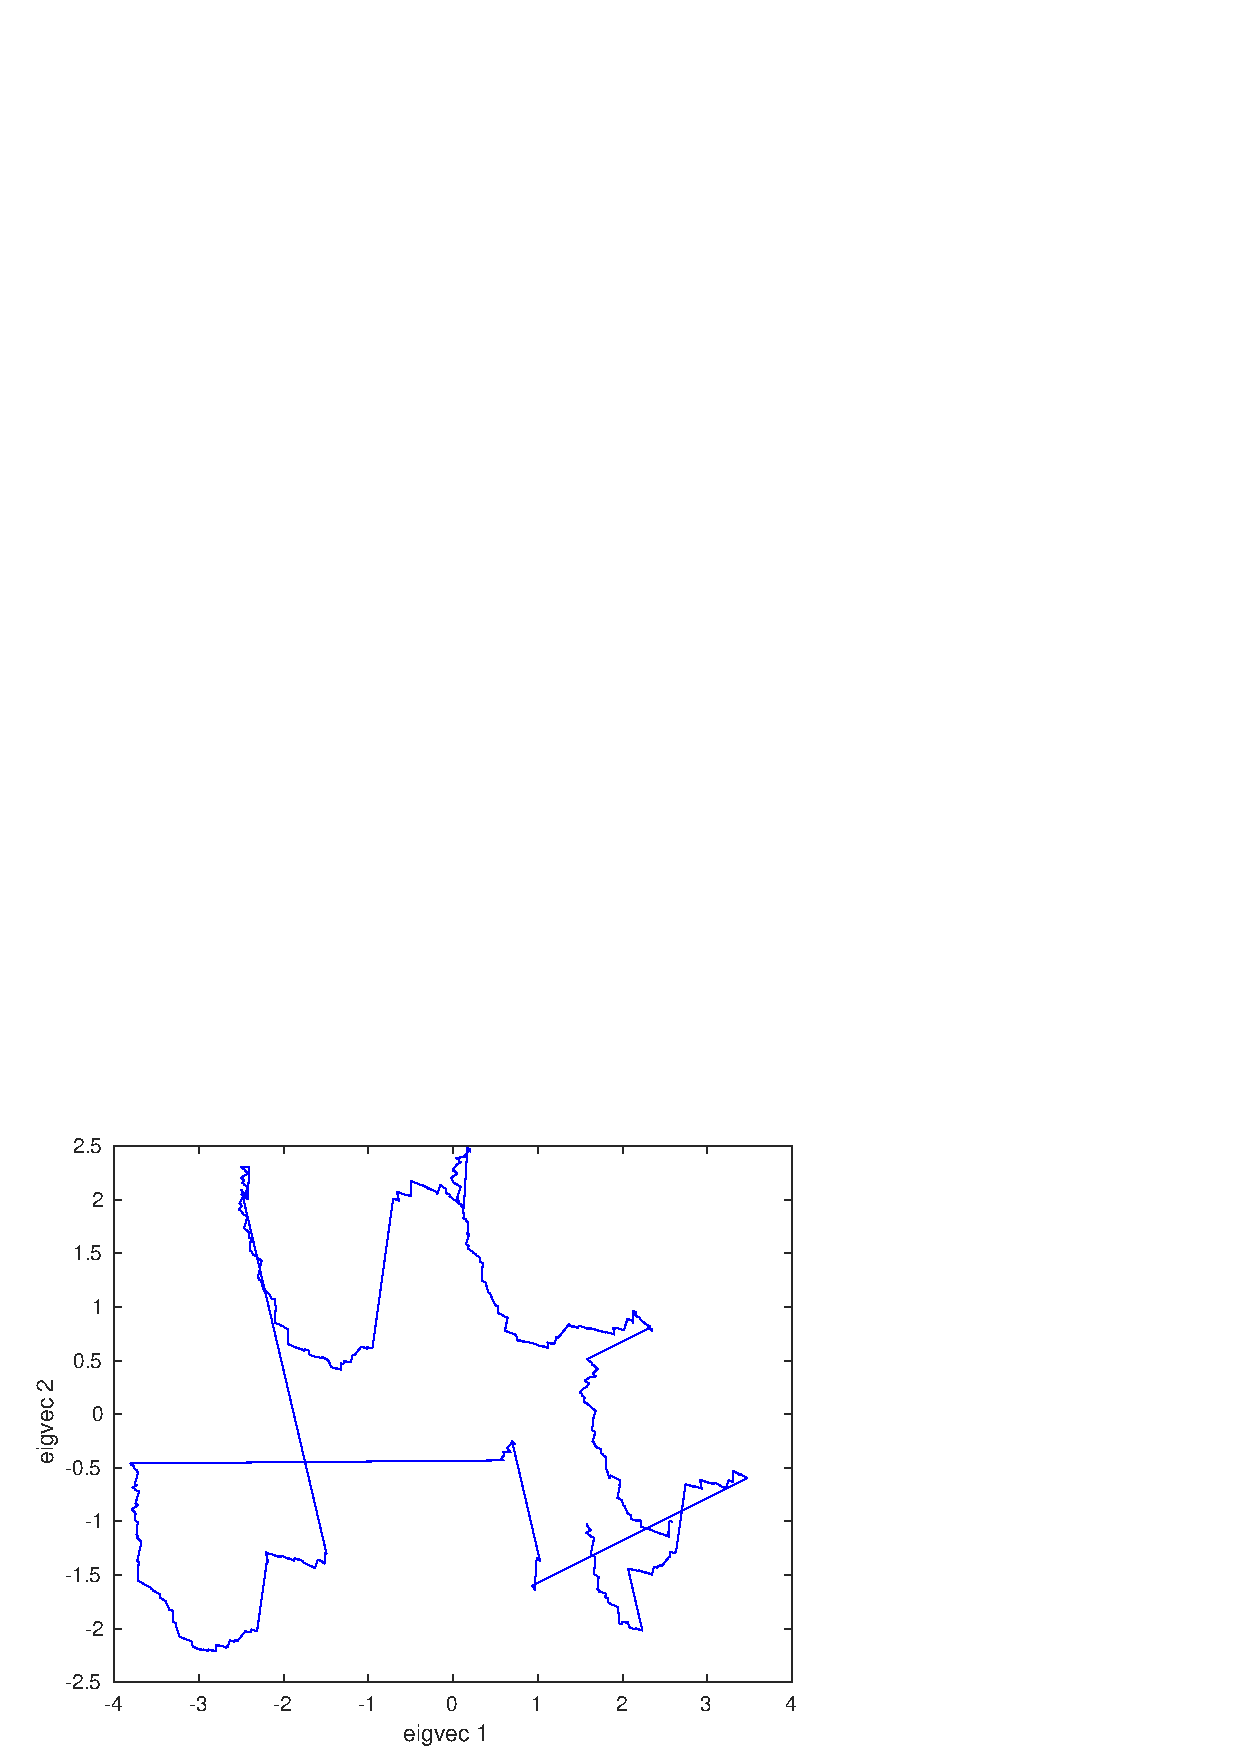
\includegraphics[width=\textwidth]{/home/tesylvia/Oral_Sept_2017/images/FinalOralPlots/SyntheticOralPaper/SimPrevtimePCA.pdf}
            \caption[]%
            {{\small PCA on Prevtime}}    
            \label{fig:PCA on Prevtime in 3D}
        \end{subfigure}
        \quad
        \begin{subfigure}[b]{0.475\textwidth}   
            \centering 
            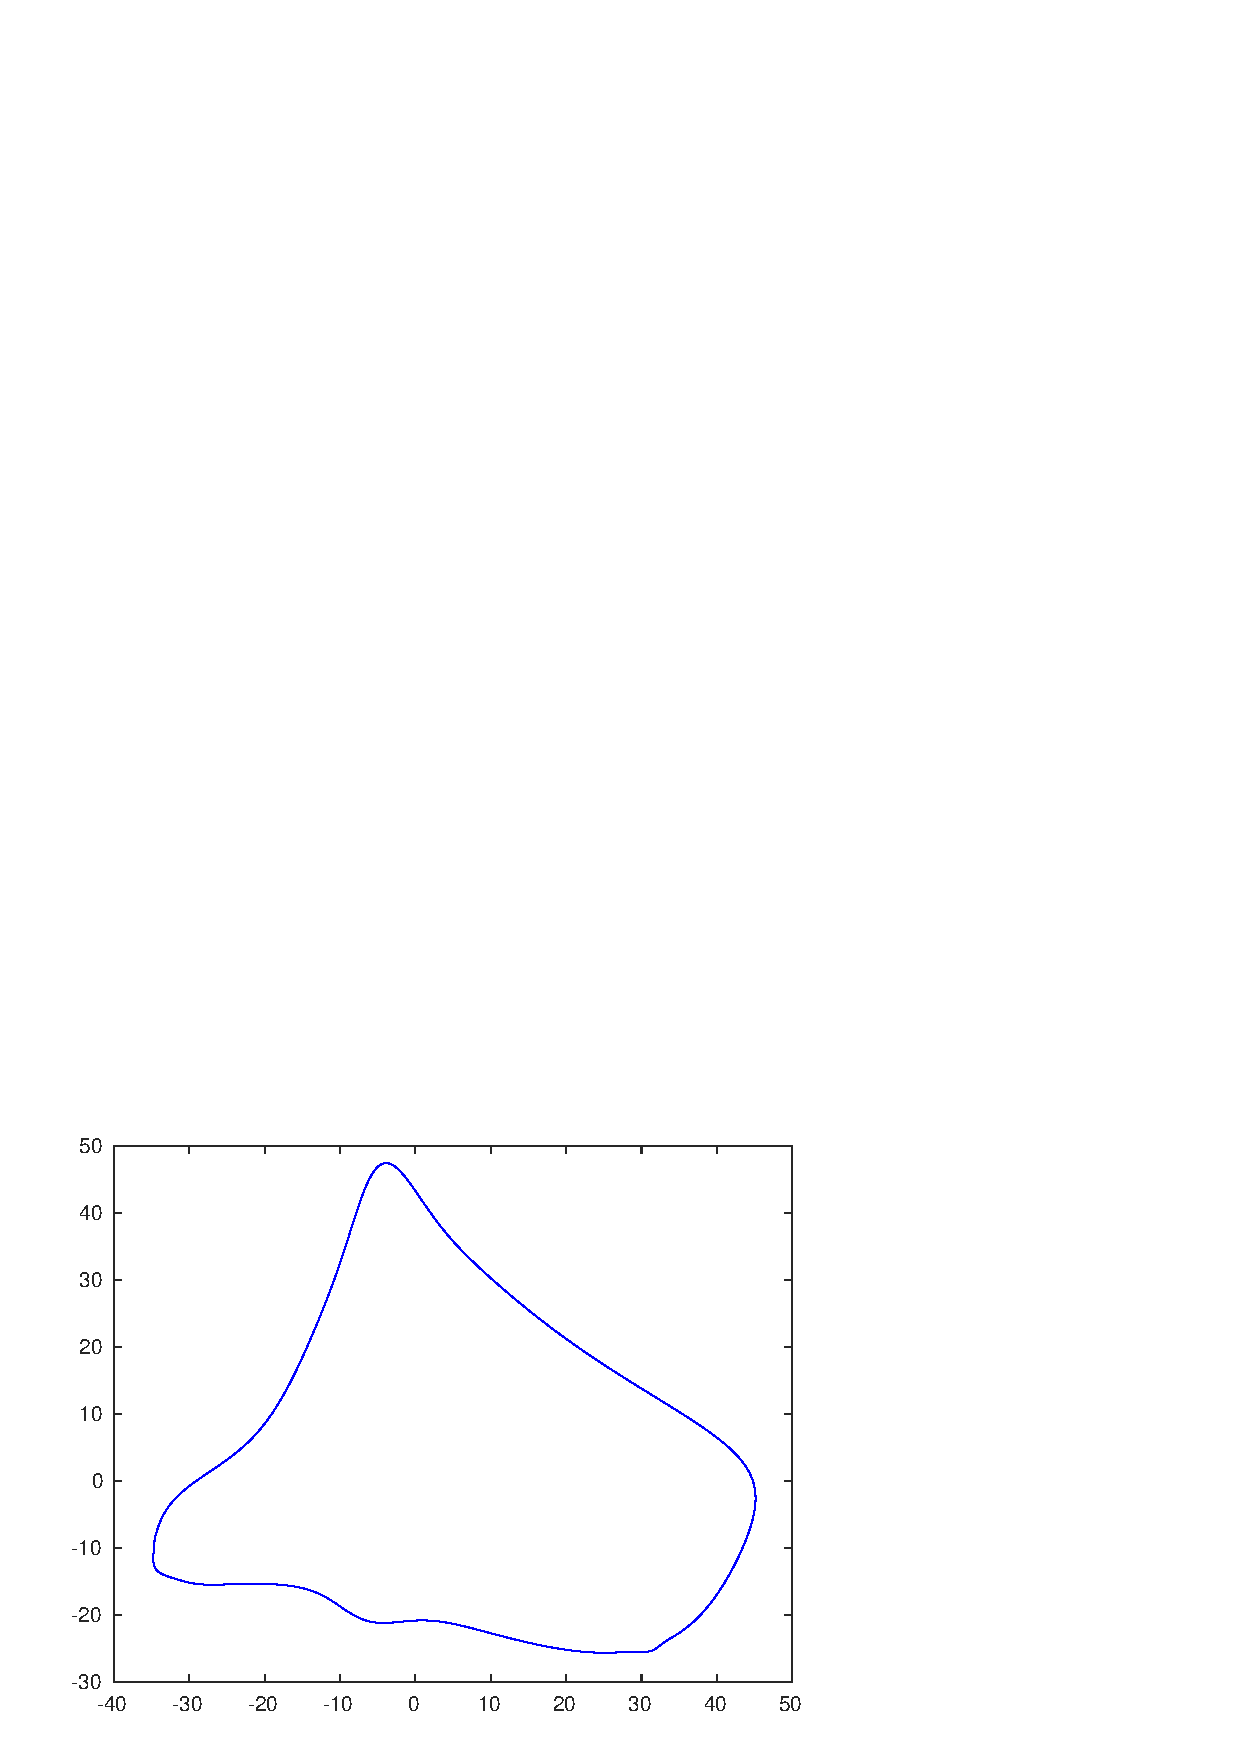
\includegraphics[width=\textwidth]{/home/tesylvia/Oral_Sept_2017/images/FinalOralPlots/SyntheticOralPaper/SimFRPCA.pdf}
            \caption[]%
            {{\small PCA on FR}}    
            \label{fig:PCA on prevtime in 2D }
        \end{subfigure}
        \vskip\baselineskip
        \begin{subfigure}[b]{0.475\textwidth}   
            \centering 
            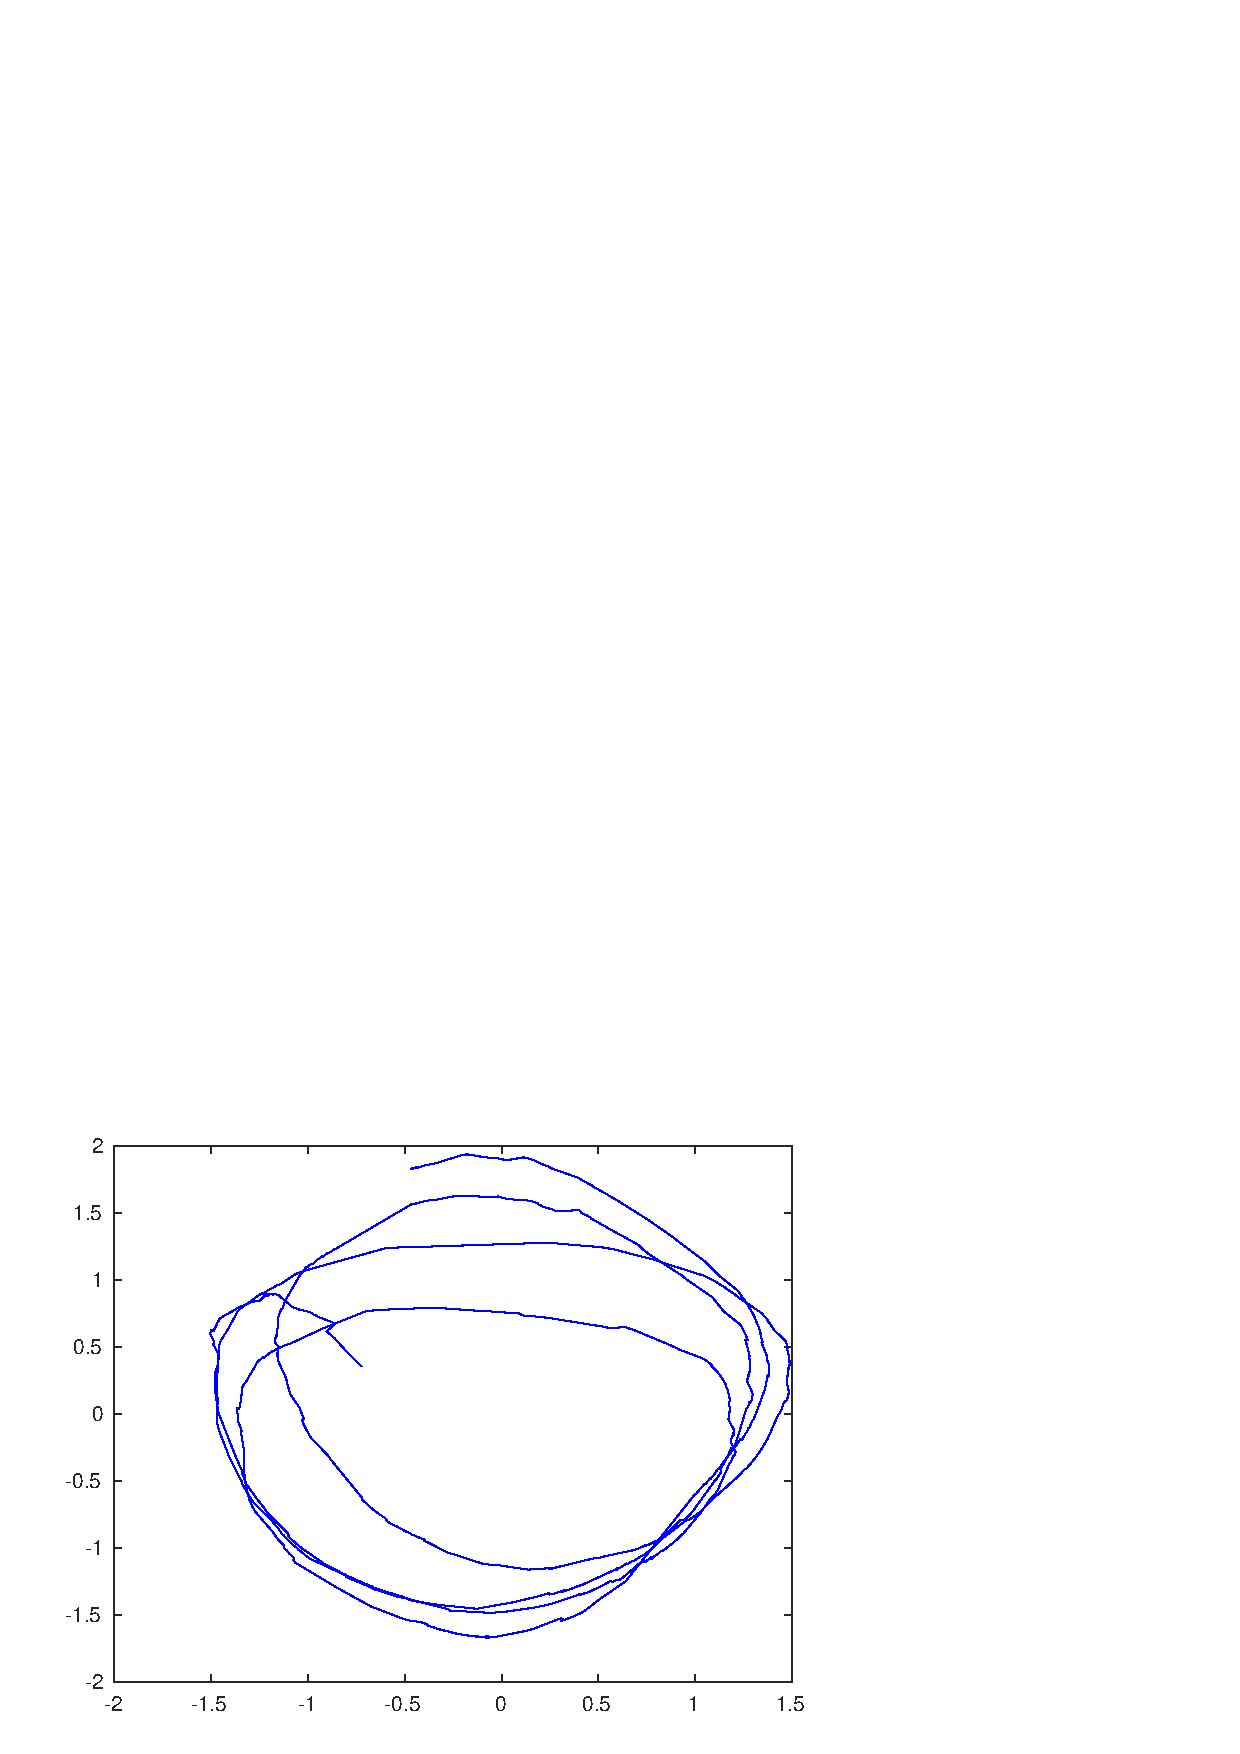
\includegraphics[width=\textwidth]{/home/tesylvia/Oral_Sept_2017/images/FinalOralPlots/SyntheticOralPaper/SimPrevtimeDML1.pdf}
            \caption[]%
            {{\small Diffusion Maps on Prevtime}}    
            \label{fig:Diffusion maps on Prevtime in 3D}
        \end{subfigure}
        \quad
        \begin{subfigure}[b]{0.475\textwidth}   
            \centering 
            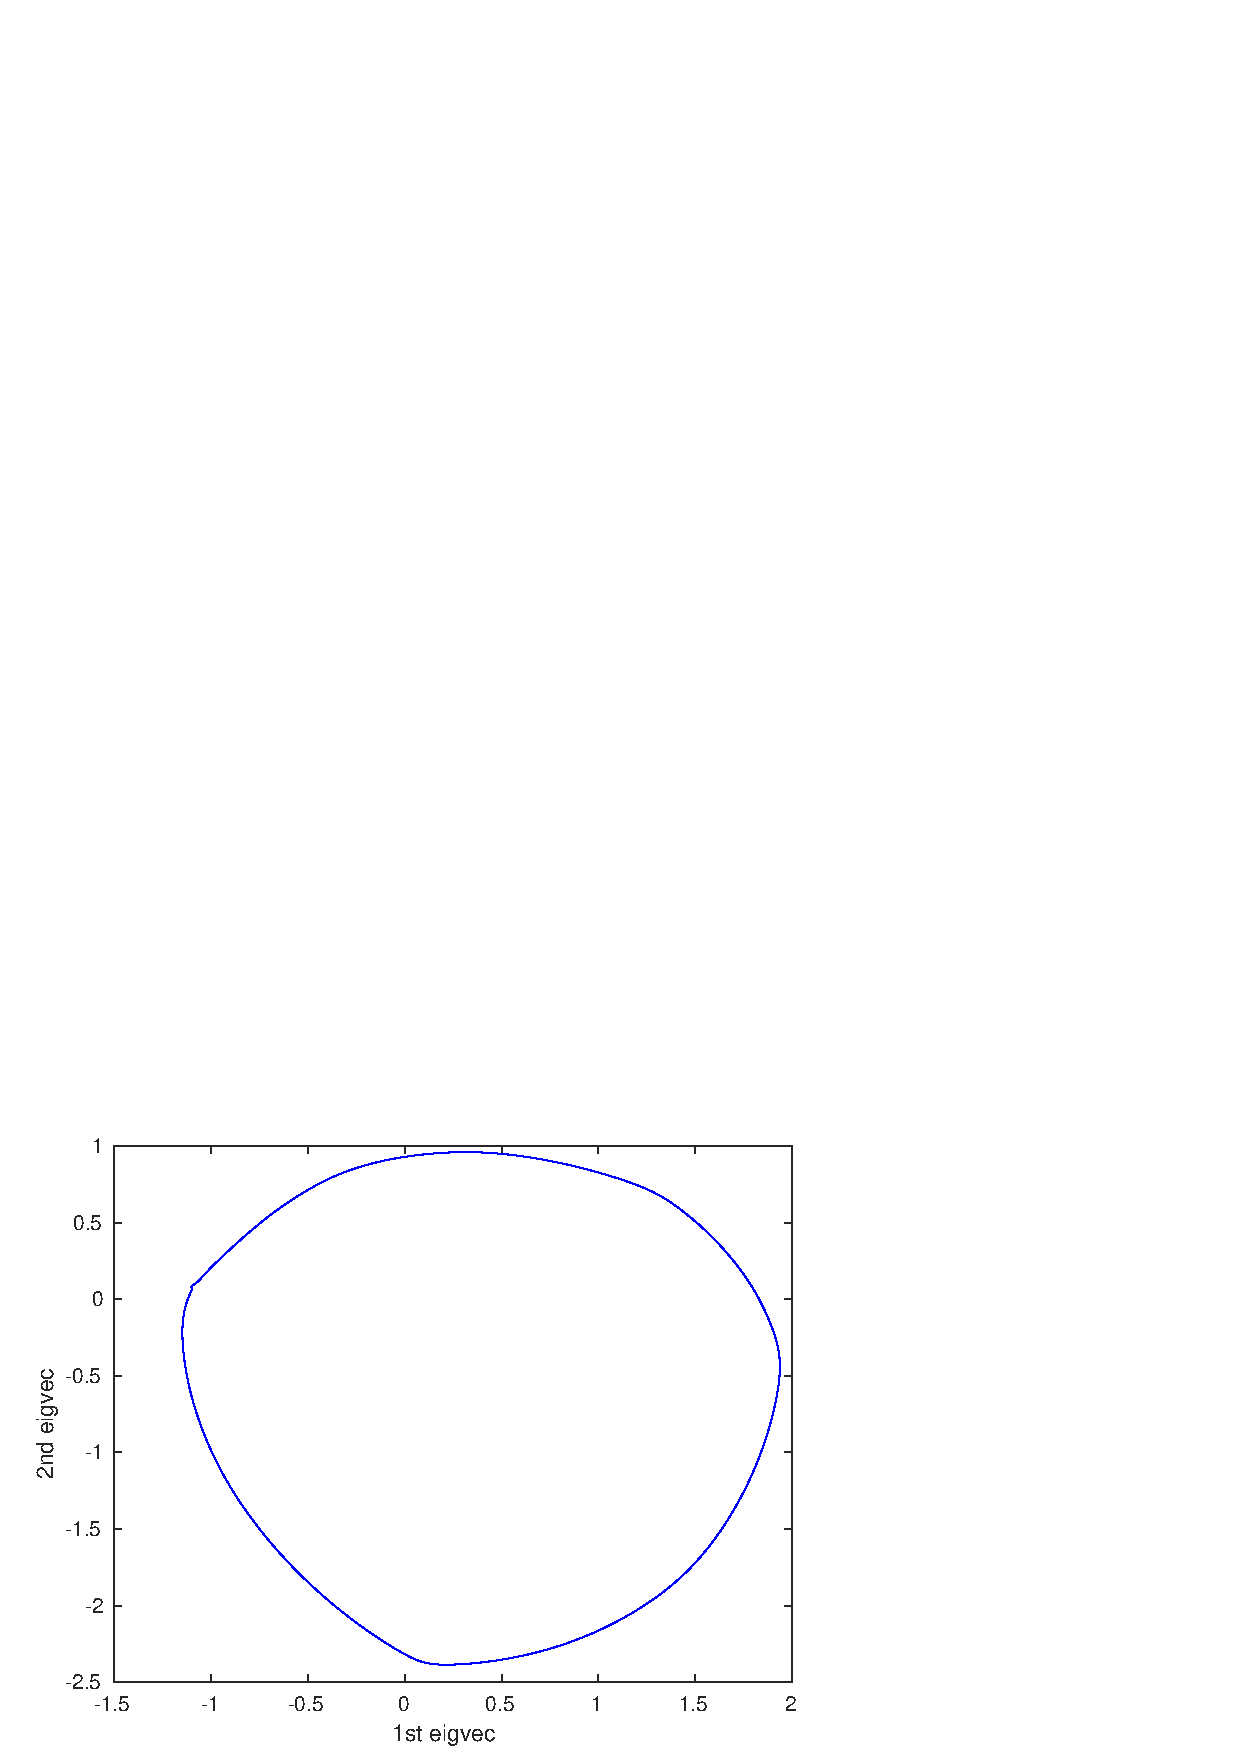
\includegraphics[width=\textwidth]{/home/tesylvia/Oral_Sept_2017/images/FinalOralPlots/SyntheticOralPaper/SimFRDML1.pdf}
            \caption[]%
            {{\small Diffusion Maps on FR}}    
            \label{fig:Diffusion maps on Prevtime in 3D }
        \end{subfigure}
        \caption[Performance of Diffusion maps and PCA on data ]
        {\small Performance of Diffusion maps and PCA on simulated previous time data (left column) and on simulated firing rate data (right column).} 
        \label{fig:DiffMaps_PCA_on_Prevtime_FR}
\end{figure}



















%\newpage

%%%%%%%%%%%%%%%%%%%%  Firing rate %%%%%%%%%%%%%%%%%%%%%%%%%%%%%%%%%%%%%%%%%%%%%%%%%%


%\begin{figure}[H]
%        \centering
%        \begin{subfigure}[b]{0.475\textwidth}
%            \centering
%            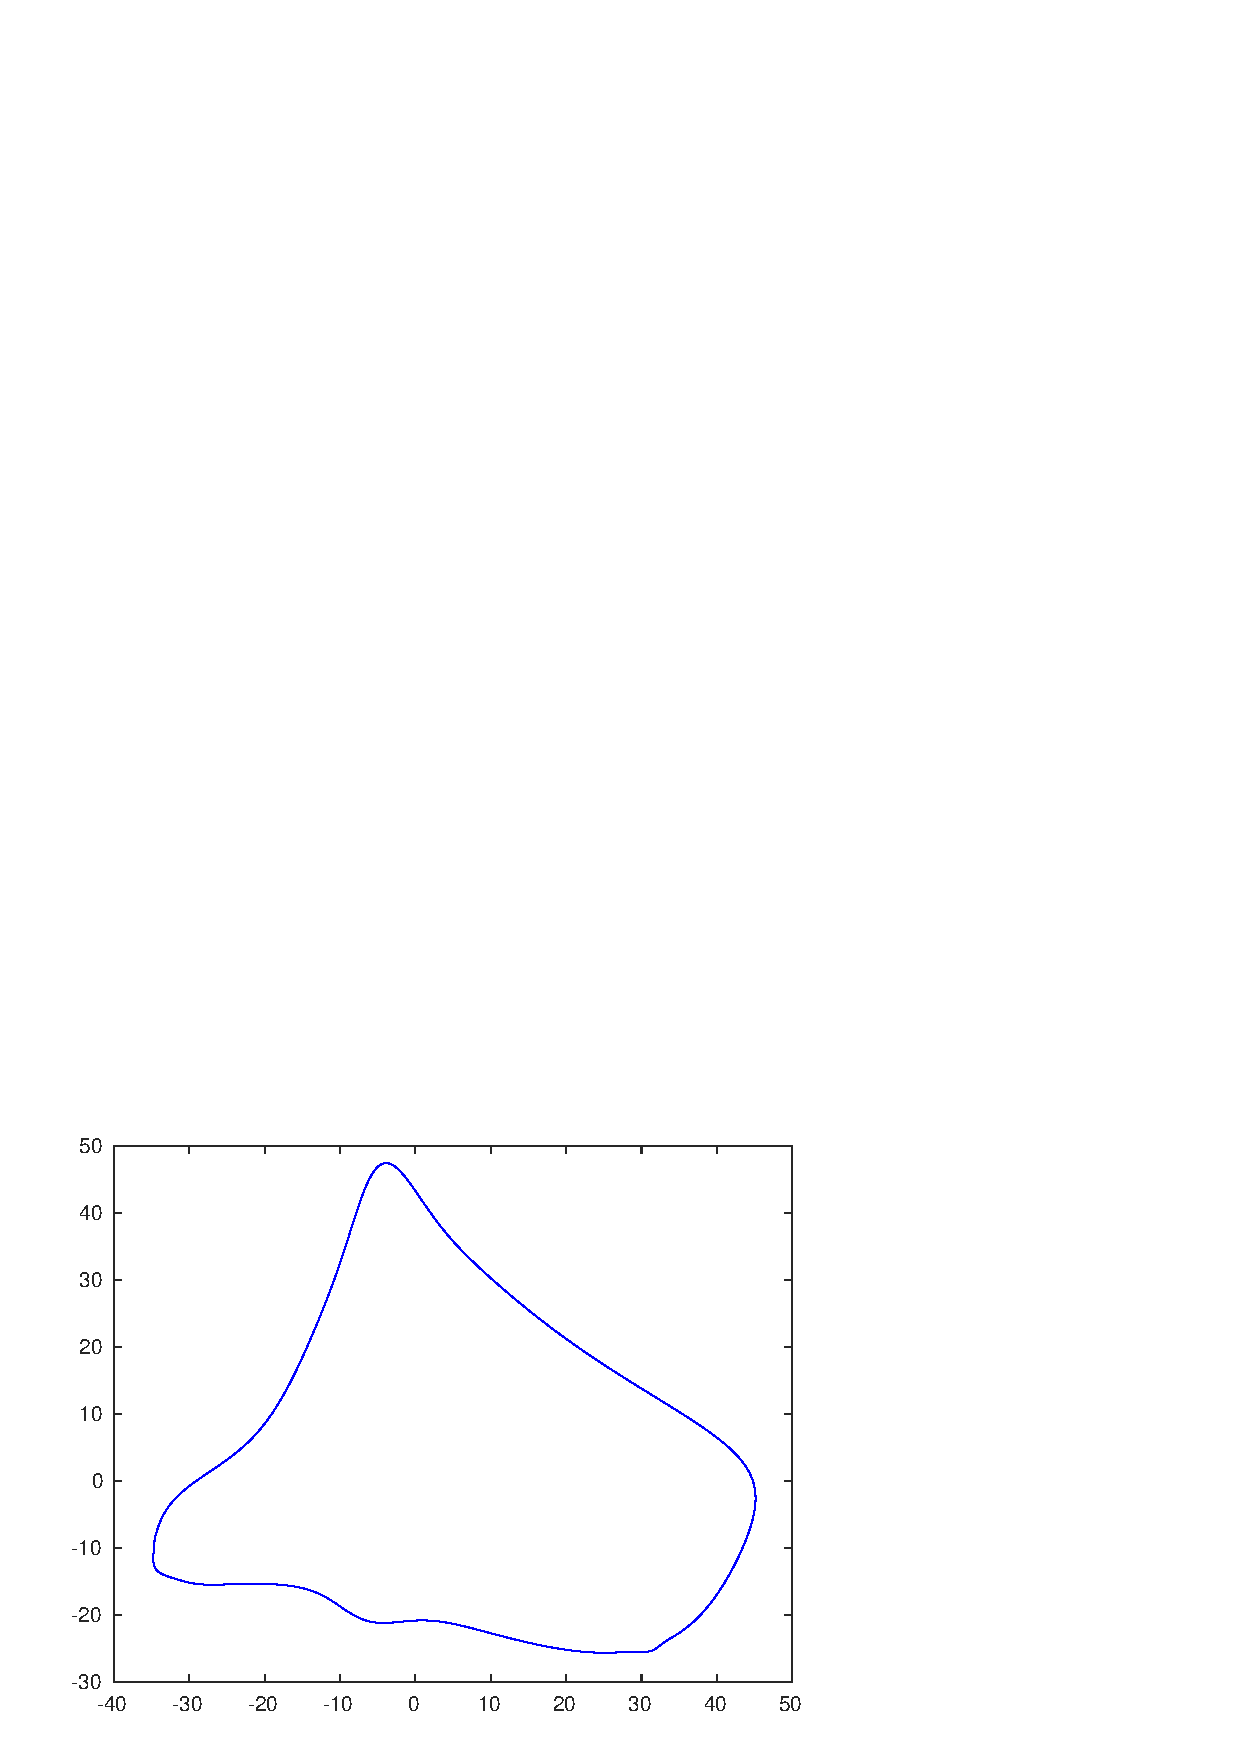
\includegraphics[width=\textwidth]{/home/tesylvia/Oral_Sept_2017/images/FinalOralPlots/SyntheticOralPaper/SimFRPCA.pdf}
%            \caption[PCA on FR]%
%            {{\small PCA on FR}}    
%            \label{fig:PCA on FR in 3D}
%        \end{subfigure}
%        \hfill
%        \begin{subfigure}[b]{0.475\textwidth}  
%            \centering 
%            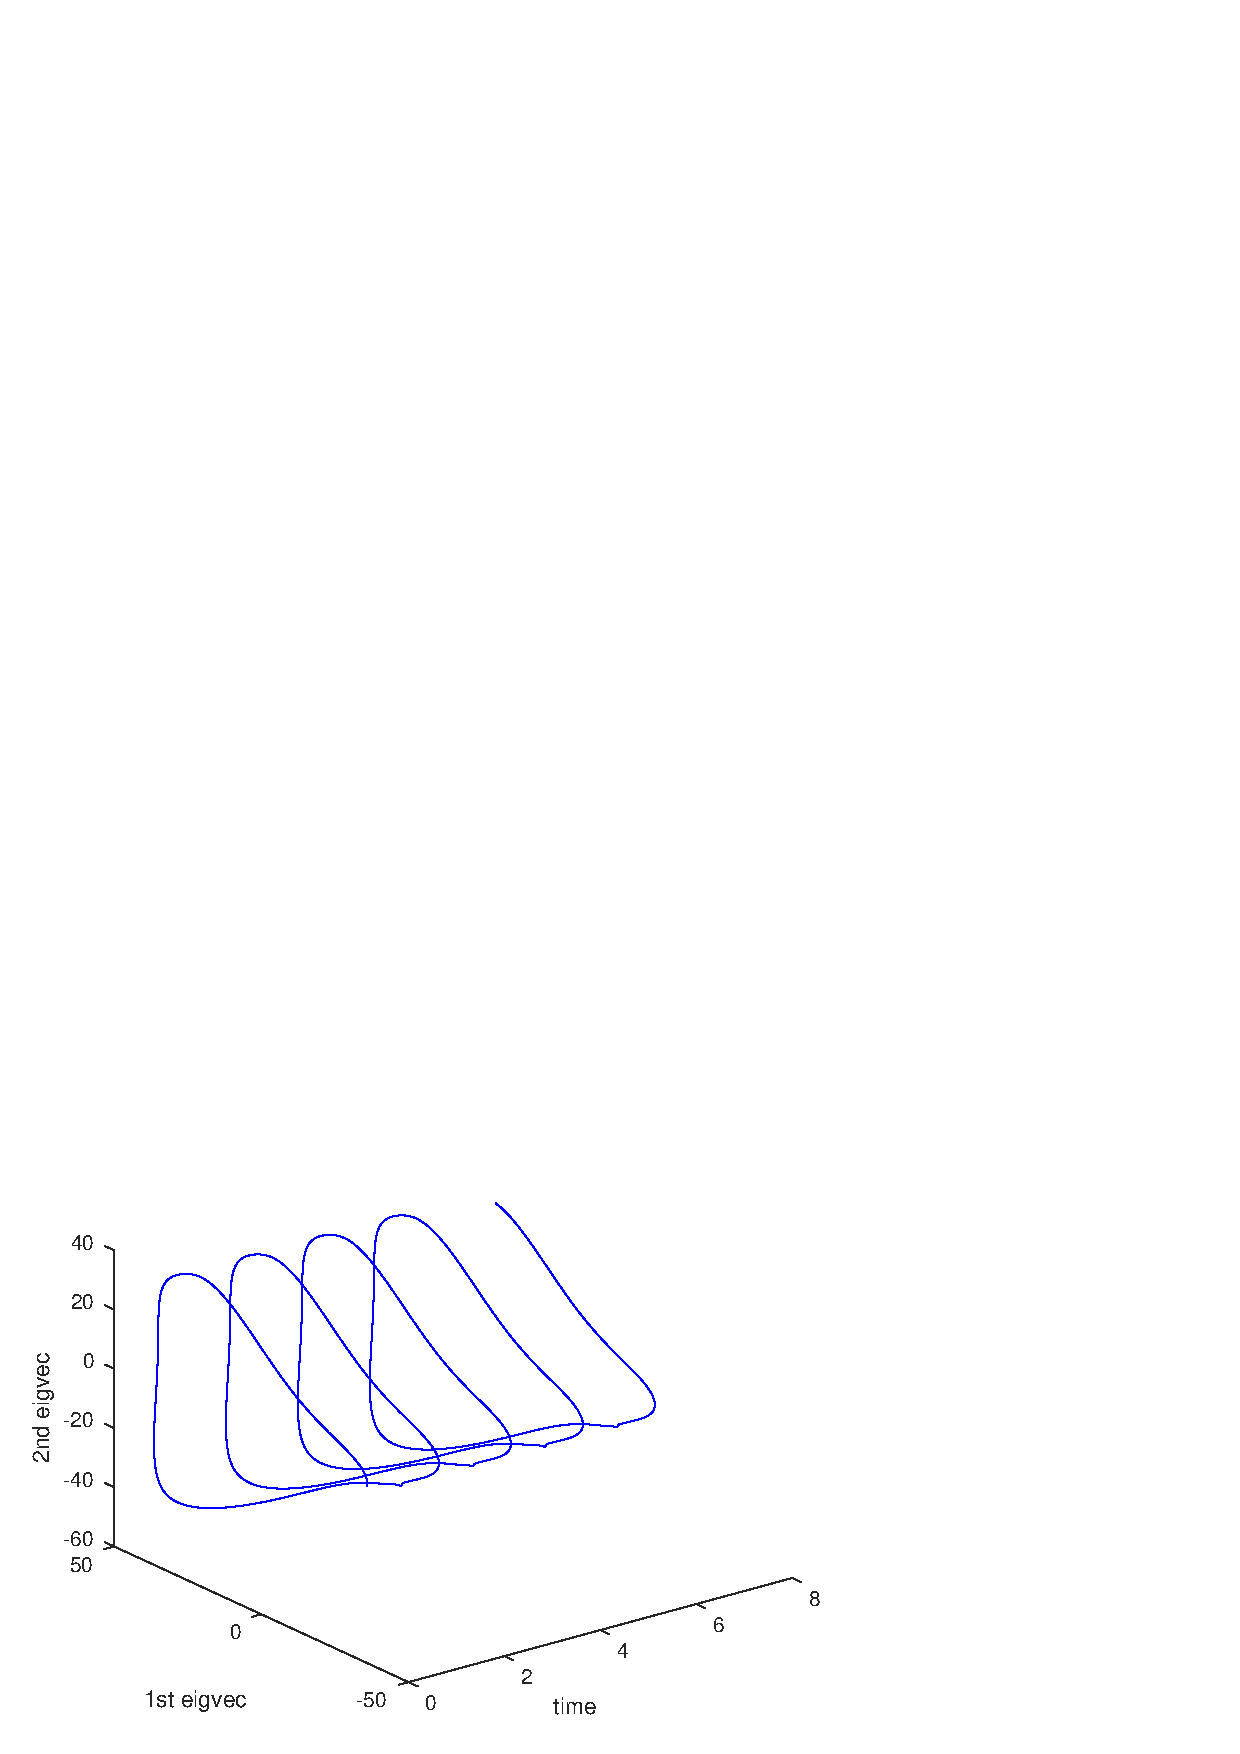
\includegraphics[width=\textwidth]{/home/tesylvia/Oral_Sept_2017/images/FinalOralPlots/SyntheticOralPaper/SimFRPCA-with-time.pdf}
%            \caption[]%
%            {{\small PCA on FR}}    
%            \label{fig:PCA on FR in 2D}
%        \end{subfigure}
%        \vskip\baselineskip
%        \begin{subfigure}[b]{0.475\textwidth}   
%            \centering 
%            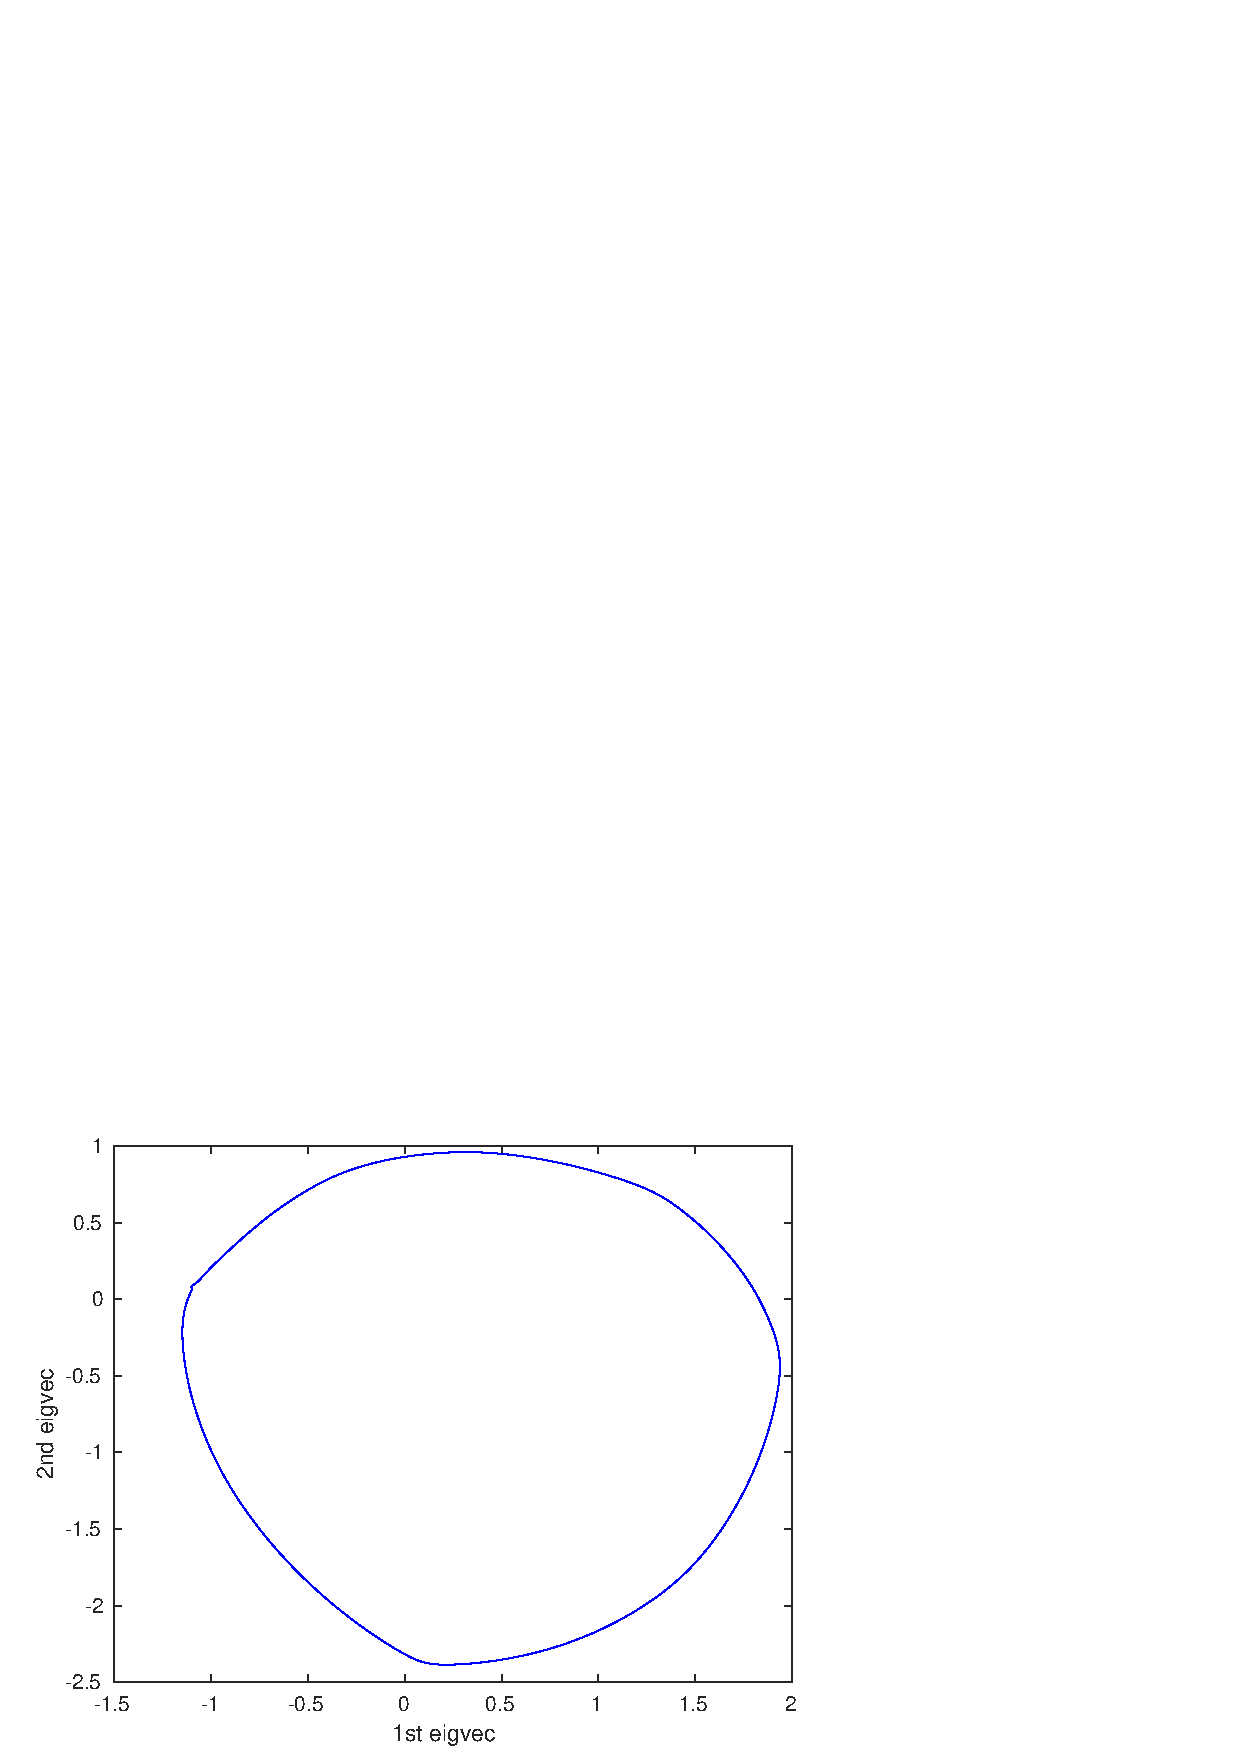
\includegraphics[width=\textwidth]{/home/tesylvia/Oral_Sept_2017/images/FinalOralPlots/SyntheticOralPaper/SimFRDML1.pdf}
%            \caption[]%
%            {{\small Diffusion Maps on FR}}    
%            \label{fig:Diffusion maps on FR in 3D}
%        \end{subfigure}
%        \quad
%        \begin{subfigure}[b]{0.475\textwidth}   
%            \centering 
%            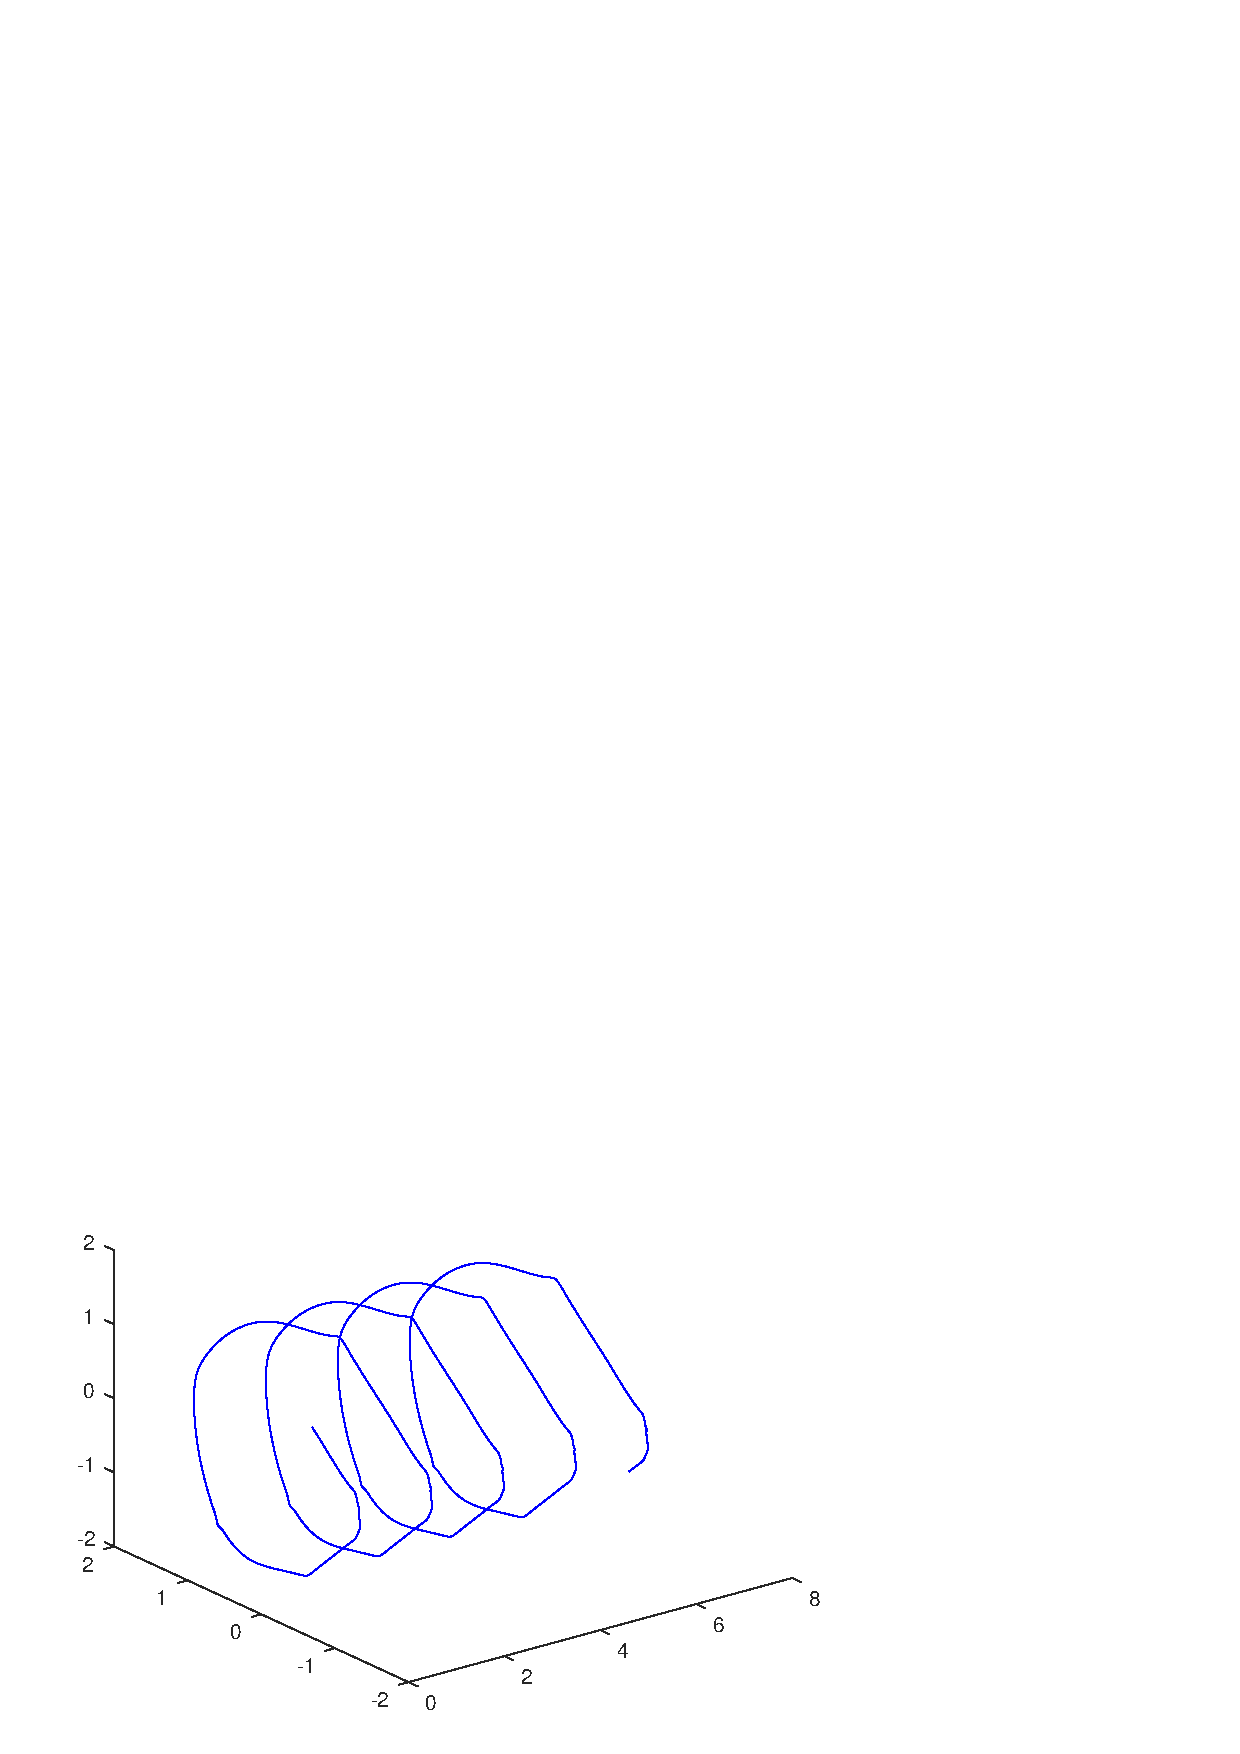
\includegraphics[width=\textwidth]{/home/tesylvia/Oral_Sept_2017/images/FinalOralPlots/SyntheticOralPaper/SimFRDML1-with-time.pdf}
%            \caption[]%
%            {{\small Diffusion Maps on FR}}    
%            \label{fig:Diffusion maps on FR in 2D }
%        \end{subfigure}
%        \caption[small Performance of Diffusion maps and PCA on simulated firing rate data ]
%        {\small Performance of Diffusion maps and PCA on simulated firing rate data} 
%        \label{fig:DiffMaps_PCA_on_FR}
%    \end{figure}
%
%


%Next, we show the results of diffusion maps with $l_{1}$ distance 
%and PCA on simulated previous time data (Prevtime). 

%%%%%%%%%%%%%%%%%%%%%%%%%%%% Prevtime and simulated position %%%%%%%%%%%%%%%%%%%%%%%%%%%%%

%\begin{figure}[H]
%        \centering
%        \begin{subfigure}[b]{0.475\textwidth}
%            \centering
%            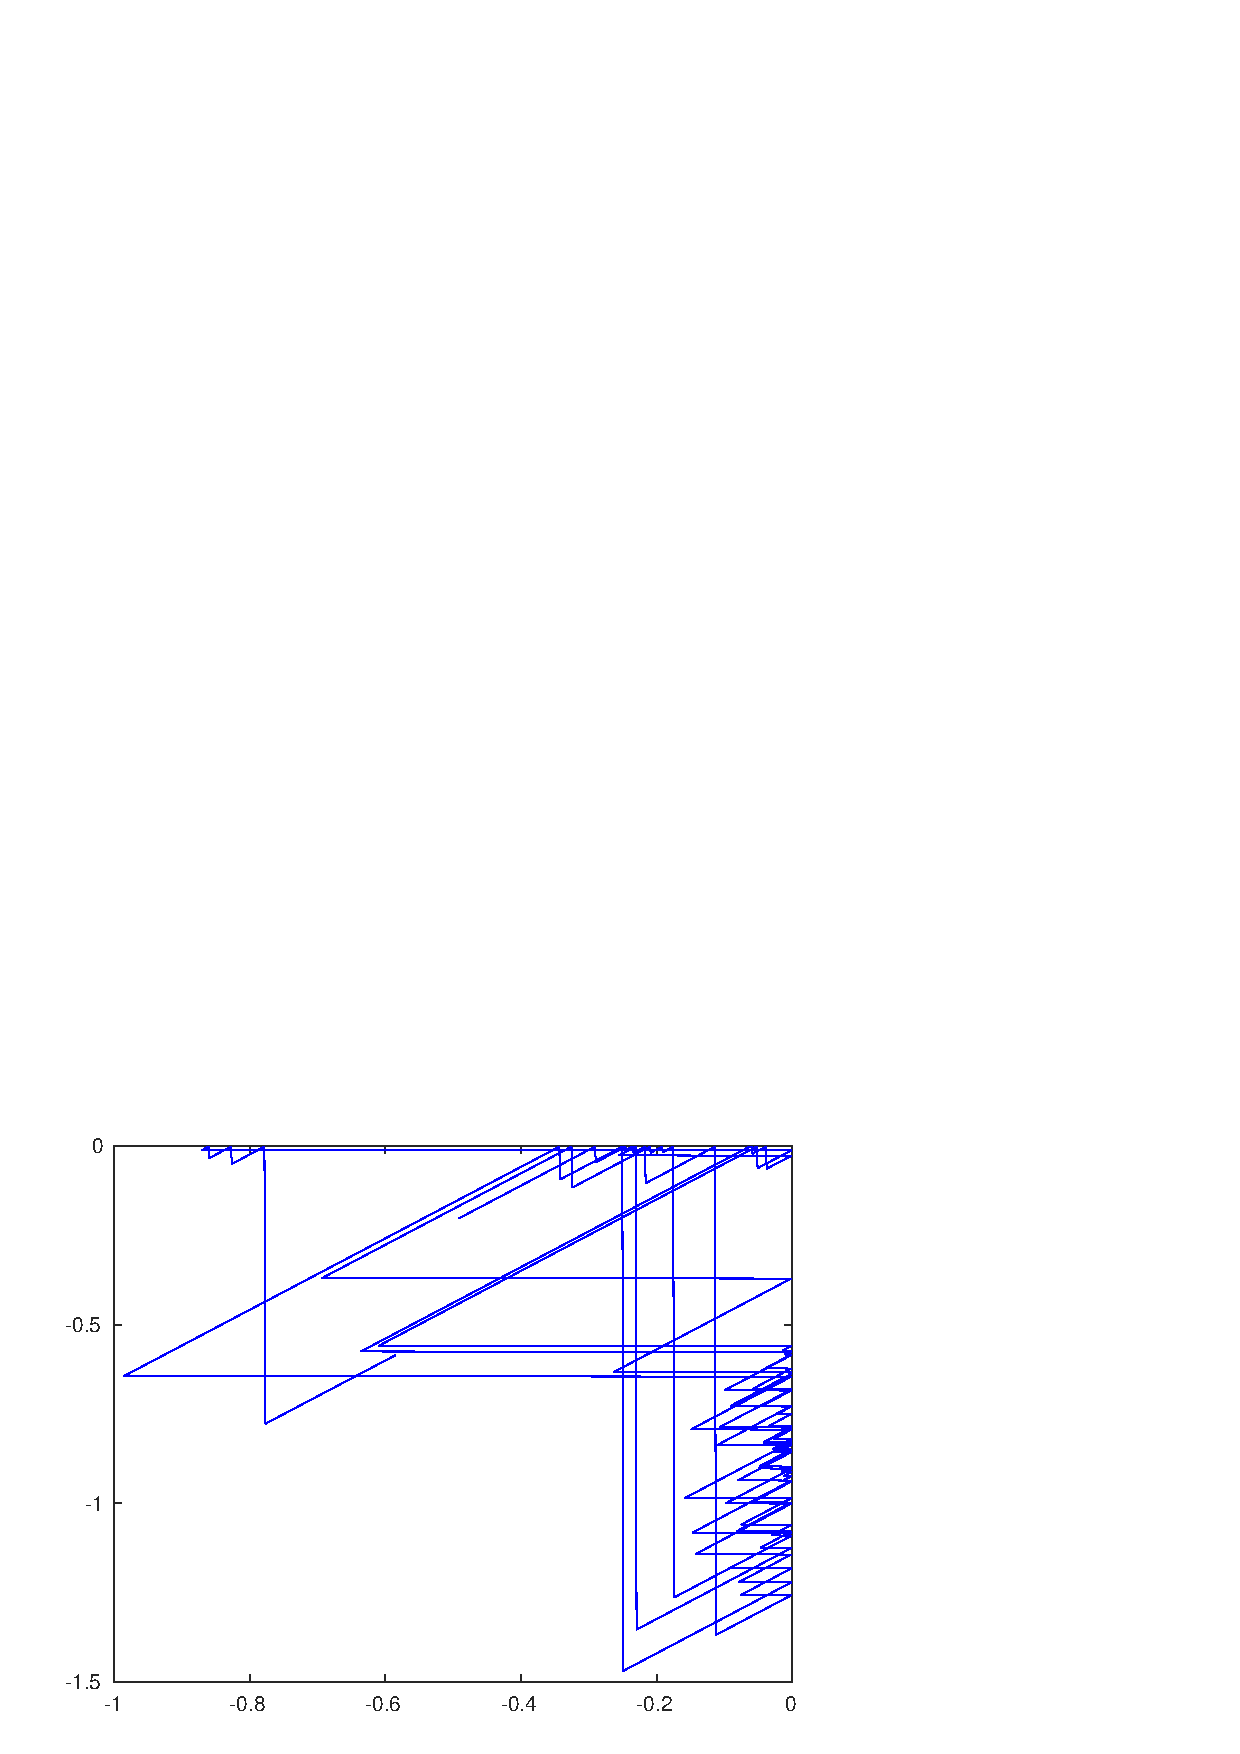
\includegraphics[width=\textwidth]{/home/tesylvia/Oral_Sept_2017/images/FinalOralPlots/SyntheticOralPaper/SimPrevtime.pdf}
%            \caption[Simulated Prevtime]%
%            {{\small Simulated Prevtime}}    
%            \label{fig:Prevtime in 3D}
%        \end{subfigure}
%        \hfill
%        \begin{subfigure}[b]{0.475\textwidth}  
%            \centering 
%            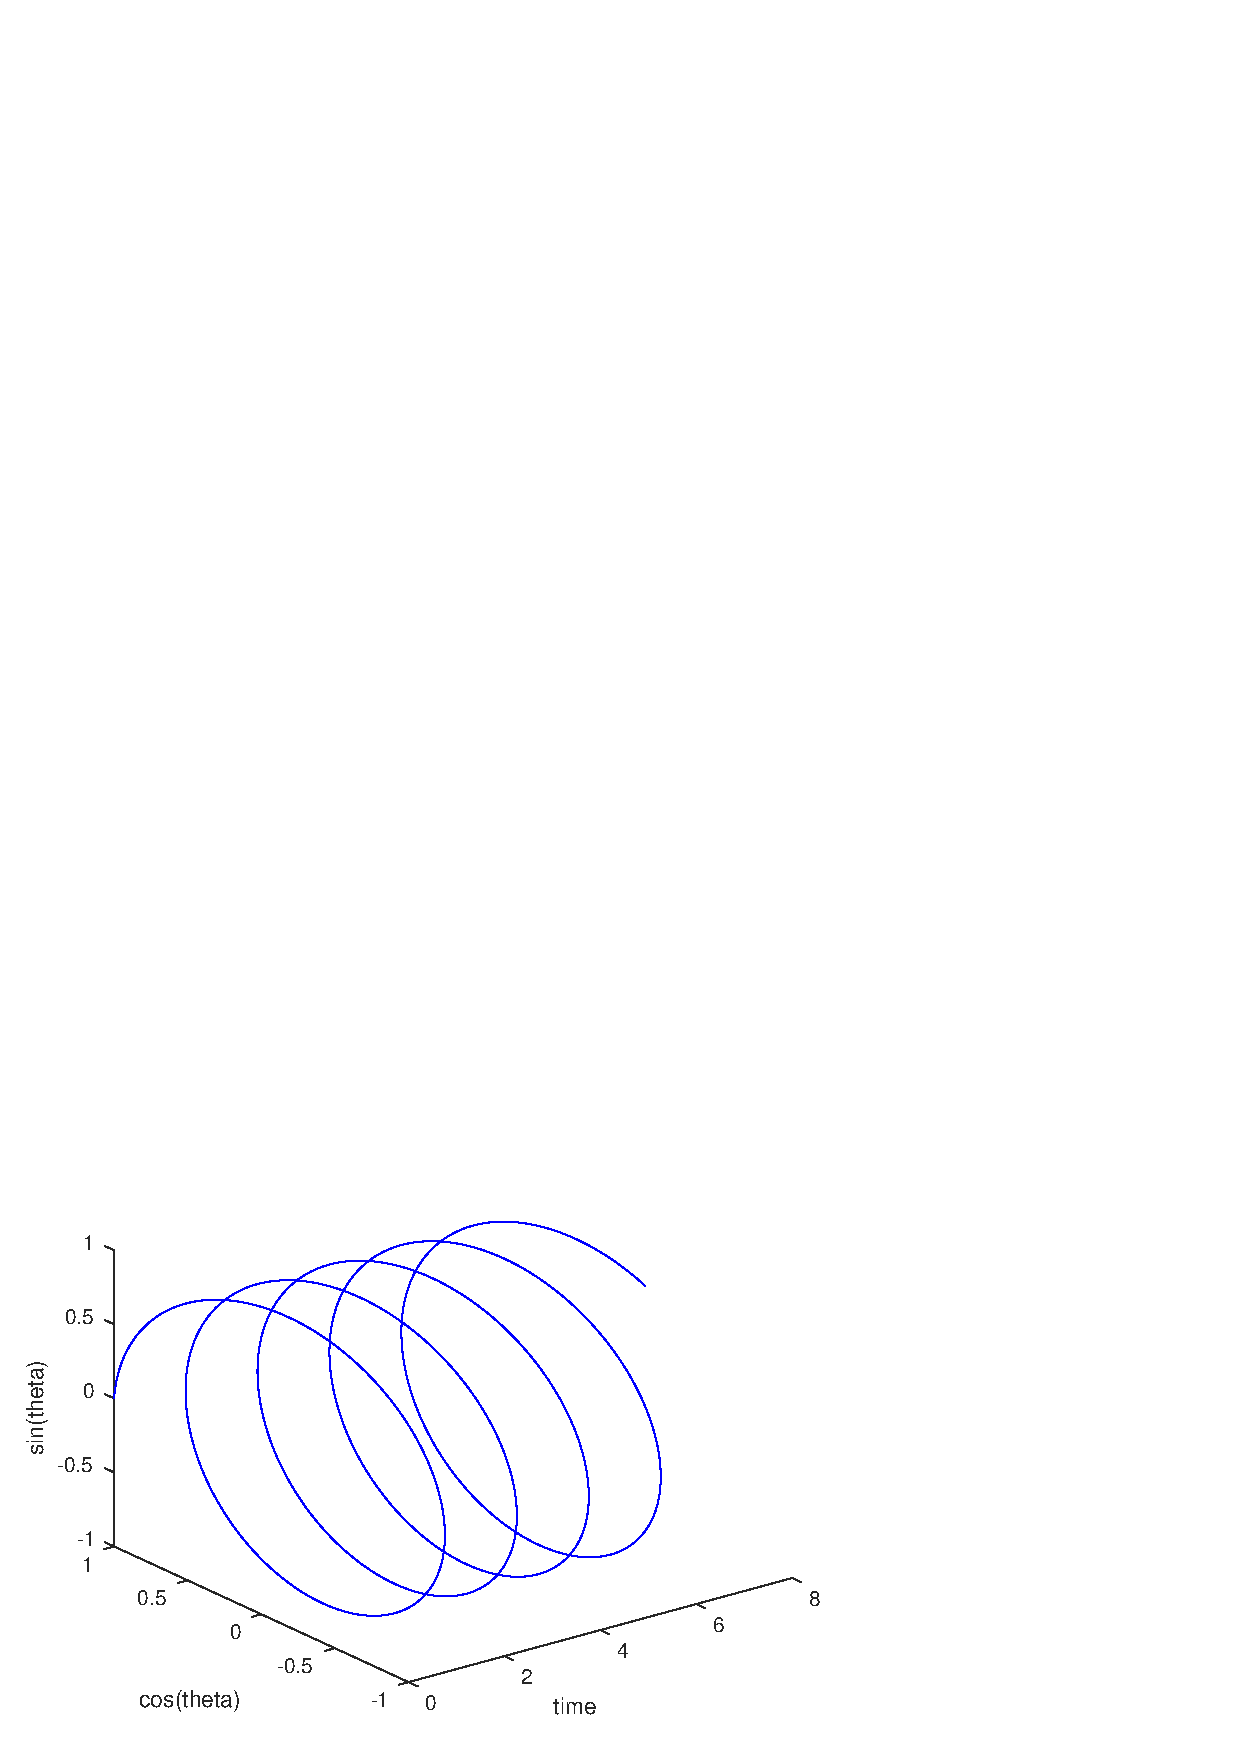
\includegraphics[width=\textwidth]{/home/tesylvia/Oral_Sept_2017/images/FinalOralPlots/SyntheticOralPaper/SimRatPosition.pdf}
%            \caption[]%
%            {{\small Simulated animal position}}    
%            \label{fig:Sim animal position in 3D}
%        \end{subfigure}
%        \vskip\baselineskip
%        \begin{subfigure}[b]{0.475\textwidth}   
%            \centering 
%            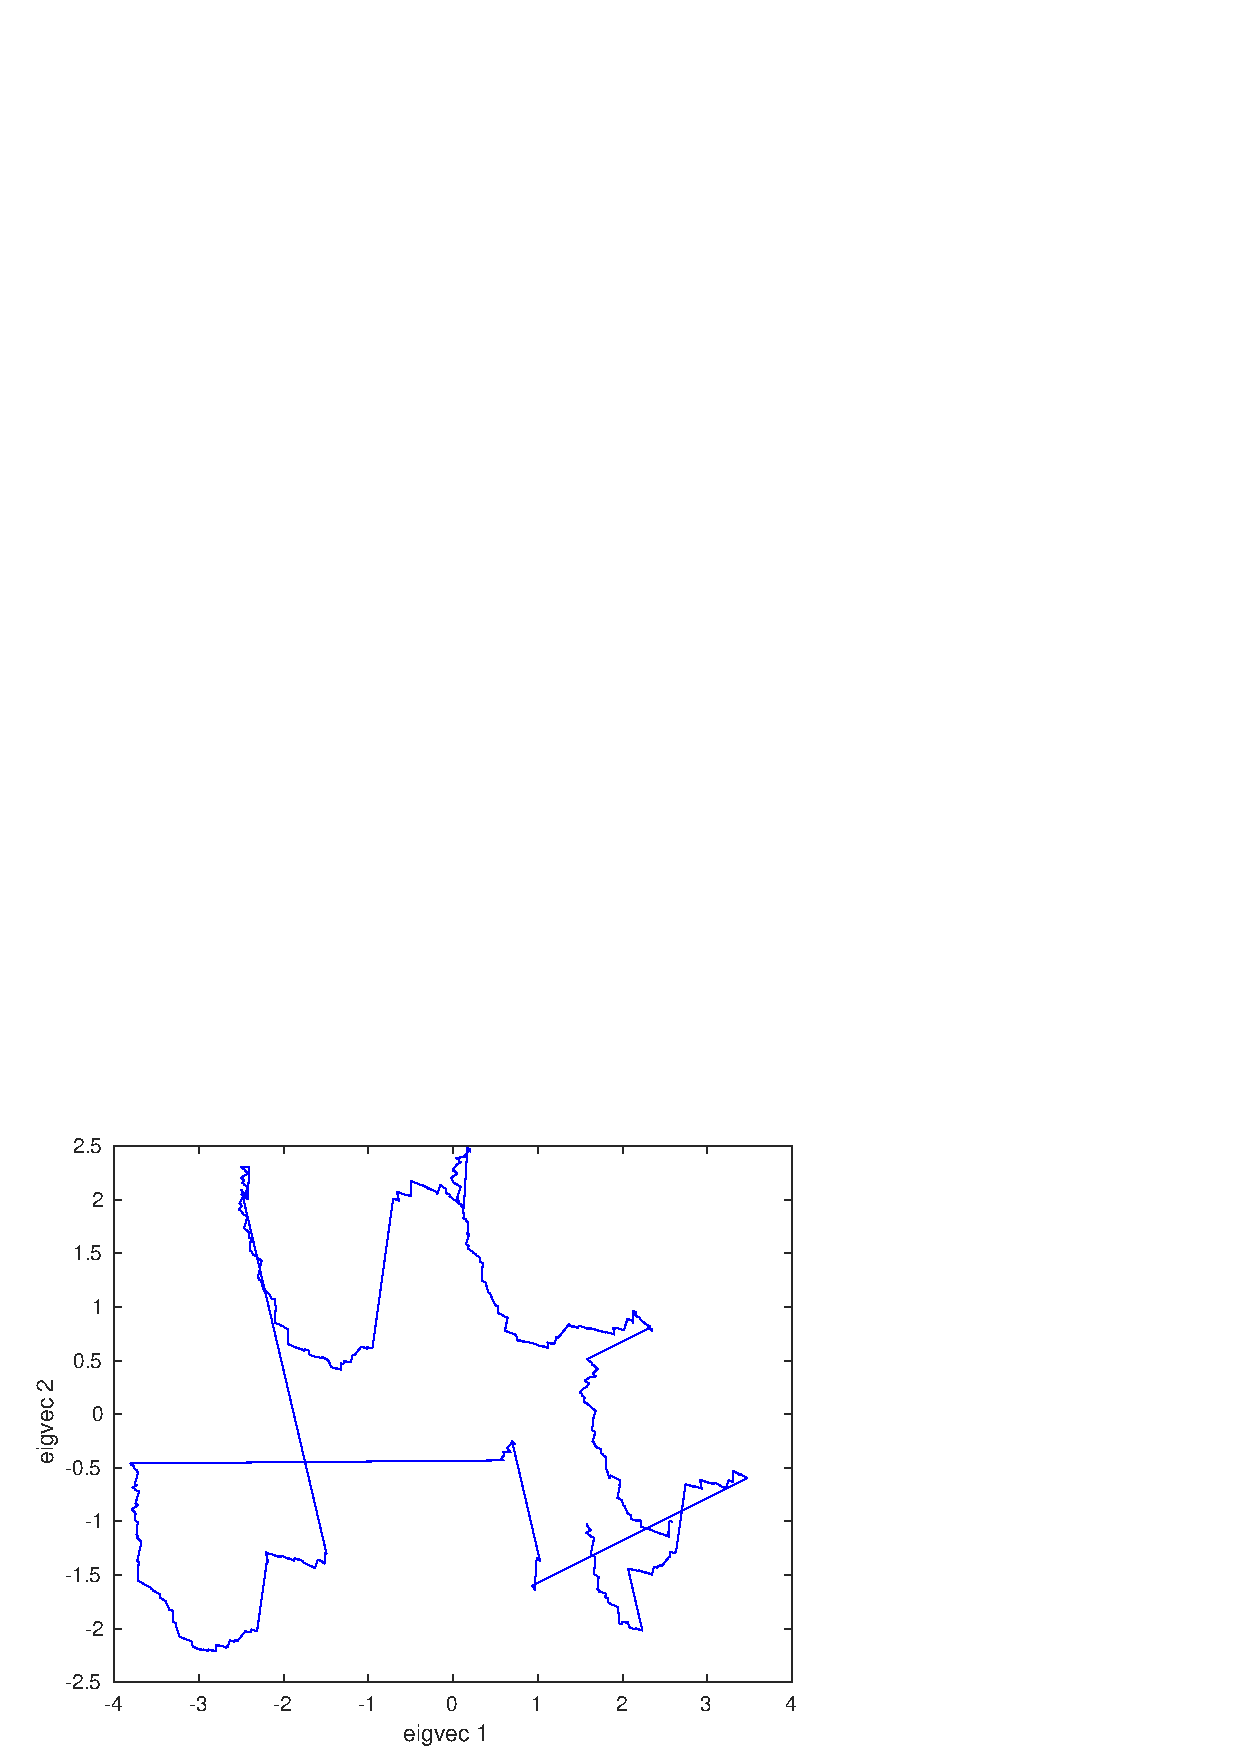
\includegraphics[width=\textwidth]{/home/tesylvia/Oral_Sept_2017/images/FinalOralPlots/SyntheticOralPaper/SimPrevtimePCA.pdf}
%            \caption[]%
%            {{\small PCA on Prevtime}}    
%            \label{fig:PCA on Prevtime in 3D}
%        \end{subfigure}
%        \quad
%        \begin{subfigure}[b]{0.475\textwidth}   
%            \centering 
%            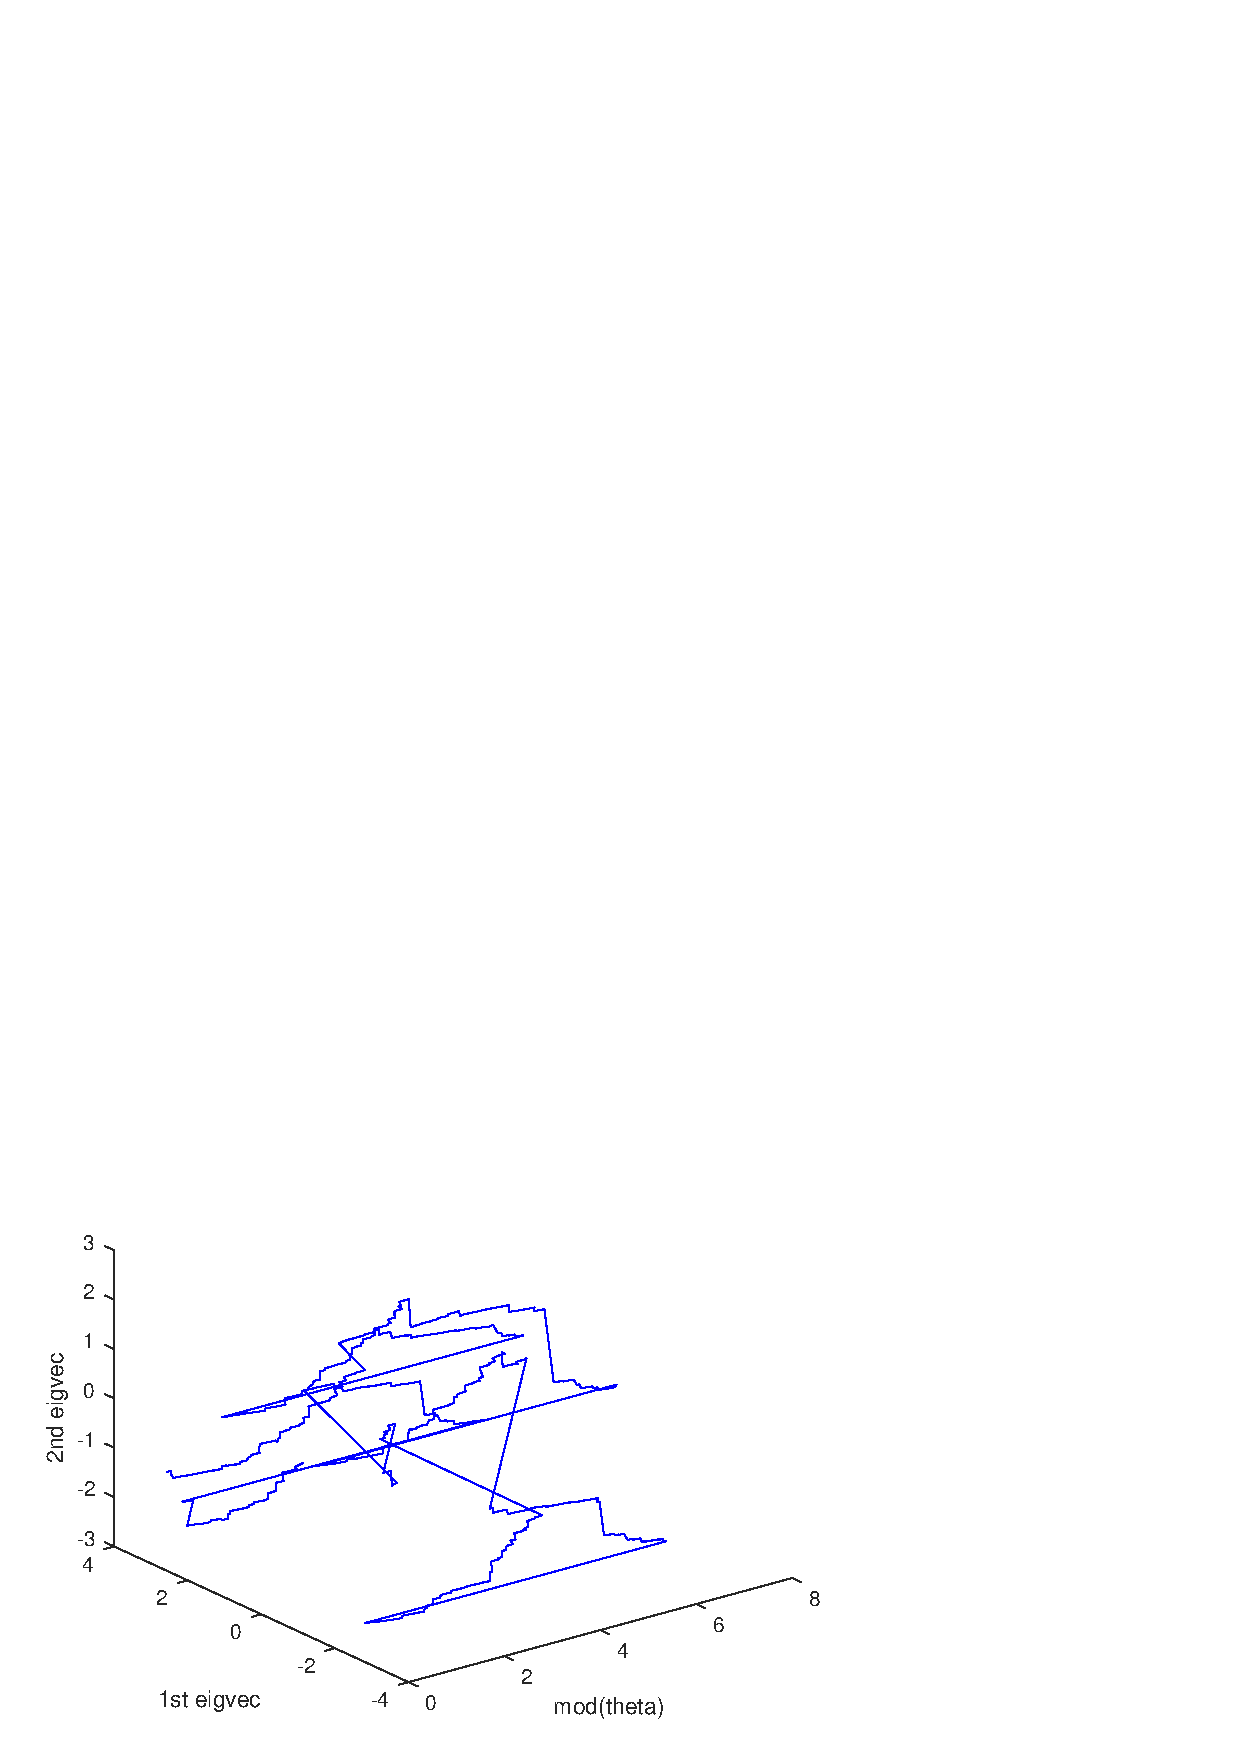
\includegraphics[width=\textwidth]{/home/tesylvia/Oral_Sept_2017/images/FinalOralPlots/SyntheticOralPaper/SimPrevtimePCA-with-Position.pdf}
%            \caption[]%
%            {{\small PCA on prevtime}}    
%            \label{fig:PCA on prevtime in 2D }
%        \end{subfigure}
%        \vskip\baselineskip
%        \begin{subfigure}[b]{0.475\textwidth}   
%            \centering 
%            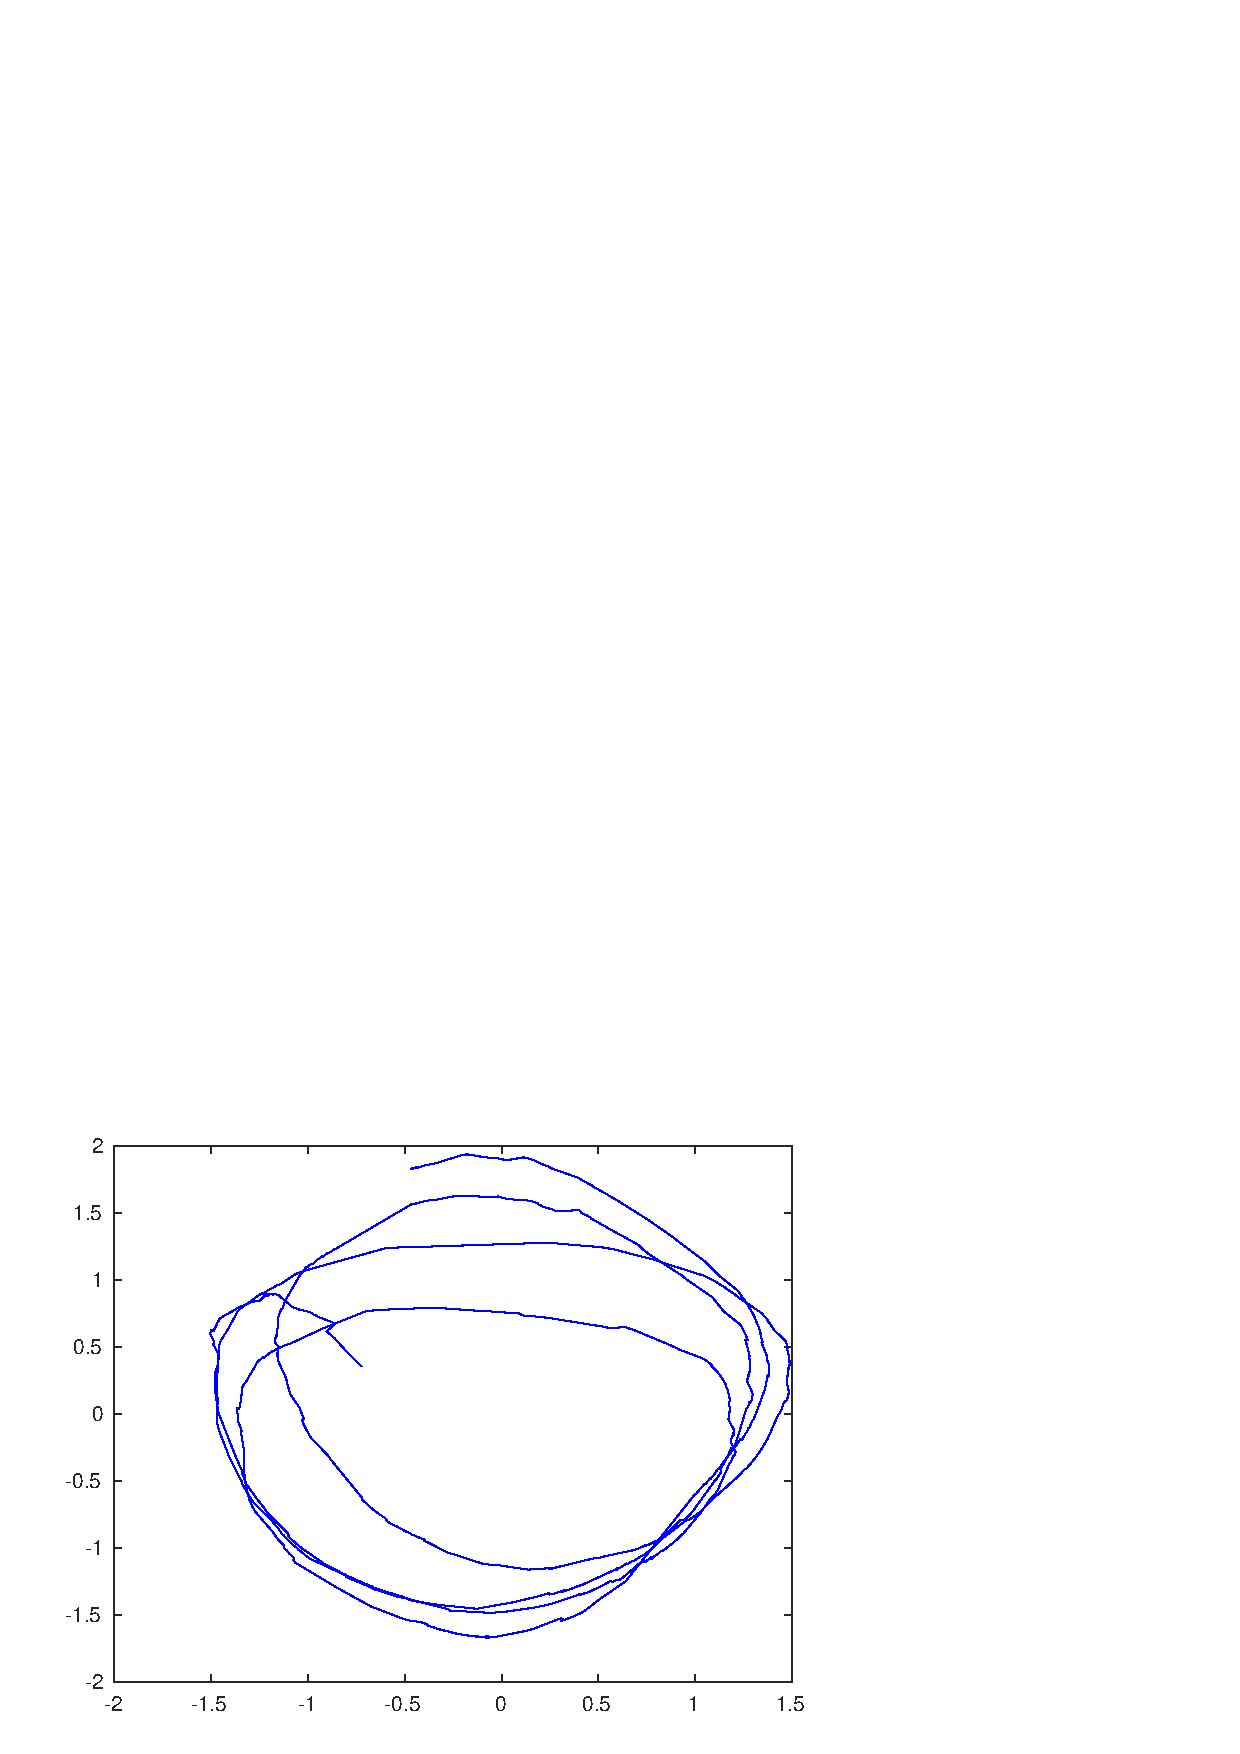
\includegraphics[width=\textwidth]{/home/tesylvia/Oral_Sept_2017/images/FinalOralPlots/SyntheticOralPaper/SimPrevtimeDML1.pdf}
%            \caption[]%
%            {{\small Diffusion Maps on Prevtime}}    
%            \label{fig:Diffusion maps on Prevtime in 3D}
%        \end{subfigure}
%        \quad
%        \begin{subfigure}[b]{0.475\textwidth}   
%            \centering 
%            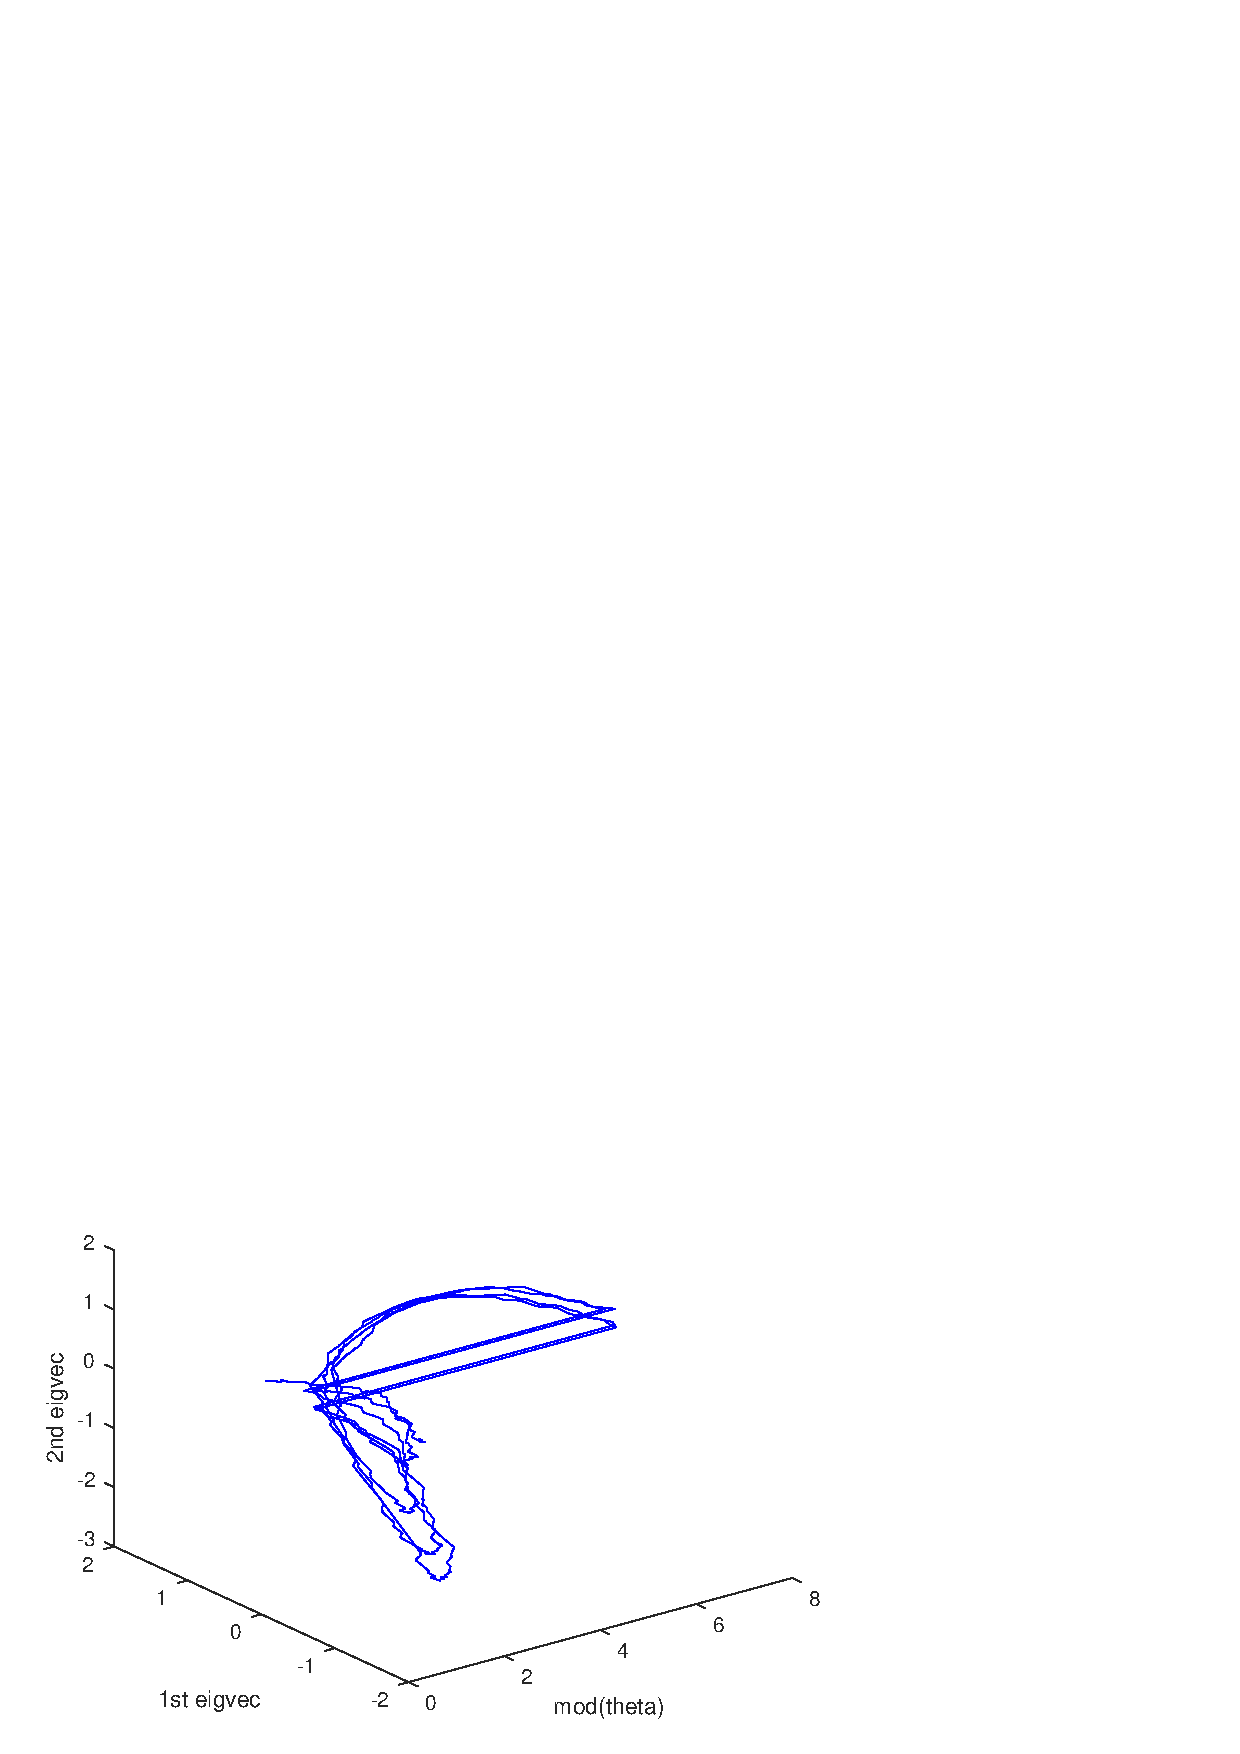
\includegraphics[width=\textwidth]{/home/tesylvia/Oral_Sept_2017/images/FinalOralPlots/SyntheticOralPaper/SimPrevtimeDML1-with-Position.pdf}
%            \caption[]%
%            {{\small Diffusion Maps on Prevtime}}    
%            \label{fig:Diffusion maps on Prevtime in 3D }
%        \end{subfigure}
%        \caption[Performance of Diffusion maps and PCA on simulated previous time data ]
%        {\small Performance of Diffusion maps and PCA on simulated previous time data} 
%        \label{fig:DiffMaps_PCA_on_Prevtime}
%\end{figure}
%


















 































































%\begin{itemize}
%\item show the graphs/results package
%\item this is how we're interpreting the results
%\item why does this matter?
%\item what measure of goodness did you use?
%(Fisher Vs Shannon information)

%%==========suggested by Duane============================================
%\item Mention that there are other ways of checking measures of goodness
% e.g the one provided by diffusion maps, Bayesian decoding refer to the nature
% and review artcicle.


%\end{itemize}







